\chapter{A Grand Apparatus}\label{ch:lhc_cms}
\begin{aquote}{Fran\c{c}ois Englert, CMS: The Art of Science, 2016}
    A glance at the ATLAS and CMS detectors at CERN reveals their beauty...
    These detectors are the modern cathedrals of the rational world created by scientists, experimentalists, and theoreticians. 
\end{aquote}

\section{The Large Hadron Collider}
The Large Hadron Collider (LHC) is the largest particle accelerator ever built. 
Its most striking feature is a 27 km ring buried 100 m beneath the Franco-Swiss border (Fig.~\ref{fig:lhc_depth}) in which two beams of protons (or heavy ions like lead), after going through several smaller stages (Fig.~\ref{fig:cern_complex}), are accelerated to 99.9999991\% of the speed of light in opposite directions. 
The beams are steered by thousands of magnets, including 1232 superconducting dipole magnets (Fig.~\ref{fig:lhc_dipole}), placed along the circumference of the ring. 
At various points, the proton beams are directed towards each other, allowing the protons to collide. 
These collision points are surrounded by enormous, multi-layered particle detectors which record snapshots of the collisions. 

The protons are accelerated in bunches of 115 billion, so when the bunches are brought together (called a ``bunch crossing''), over 200 billion protons are brought very close together.
However, only a small portion of them actually collide. 
During ``Run 2'' of the LHC from 2016 to 2018, for instance, there were 30 proton-proton collisions (e.g. Fig.~\ref{fig:normal_pu}) per bunch crossing on average, typically with only a single ``interesting'' collision (the ``primary vertex'') amongst them. % TODO: citation needed, plot or something of pileup needed
A collision is deemed interesting if it initiates a process that a physicist at the LHC wants to study (e.g. Fig.~\ref{fig:vbswh_feynman})---the non-interesting collisions are called ``pileup.'' 
To increase our odds of producing something truly interesting, the bunch crossings are spaced close together, with only 25 nanoseconds of separation. 
To put this into context, the speed of light is roughly 1 ft/ns, so the next bunch crossing will occur before the light from a screen on one side of the CMS control room can reach the eyes of someone standing on the other side (approximately 39 feet~\cite{CMSP5Layout}).
Therefore, particle detectors on the LHC must be capable of excellent resolution \textit{and} high throughput. 
That is, they must be able to resolve the particles from the primary vertex amongst the many others produced by the pileup, all within the 25 ns between bunch crossings. 

\begin{figure}[htb]
    \centering
    \subfloat{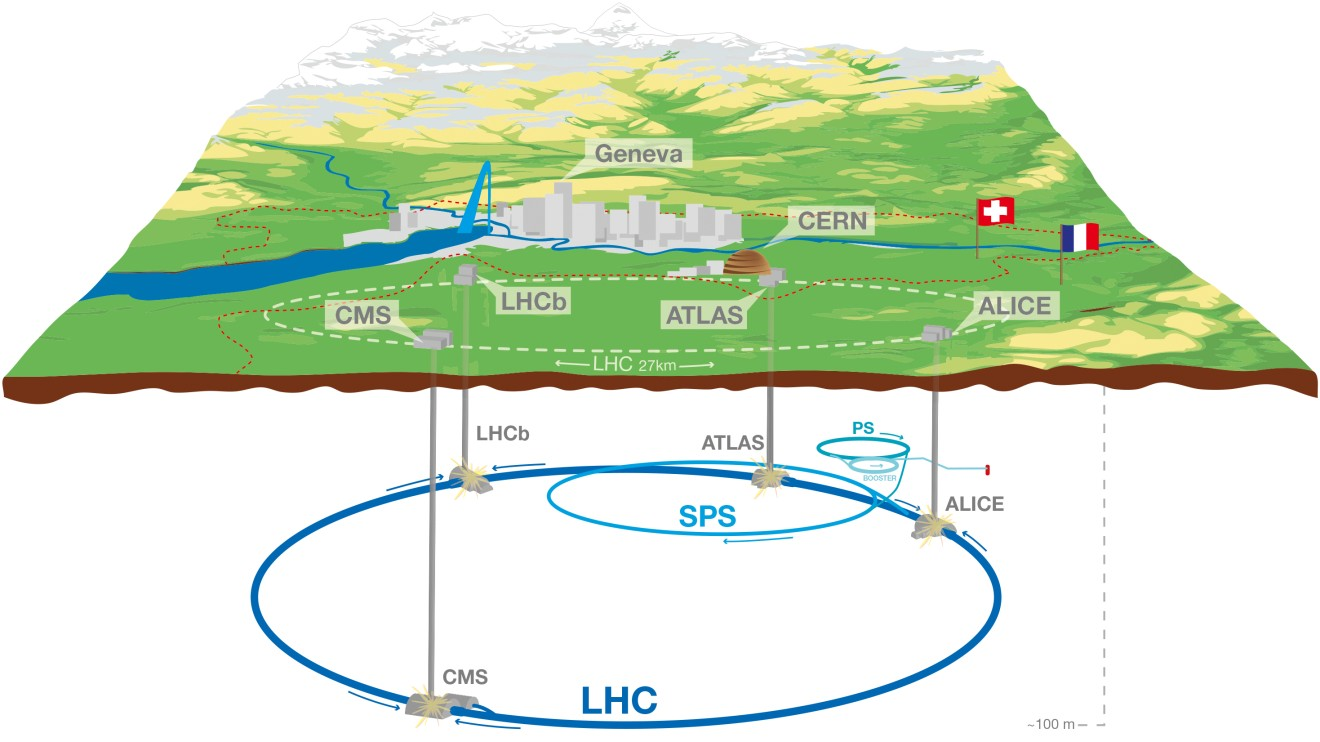
\includegraphics[width=0.45\textwidth,valign=c]{fig/lhc/lhc_depth.jpg}}\quad
    \subfloat{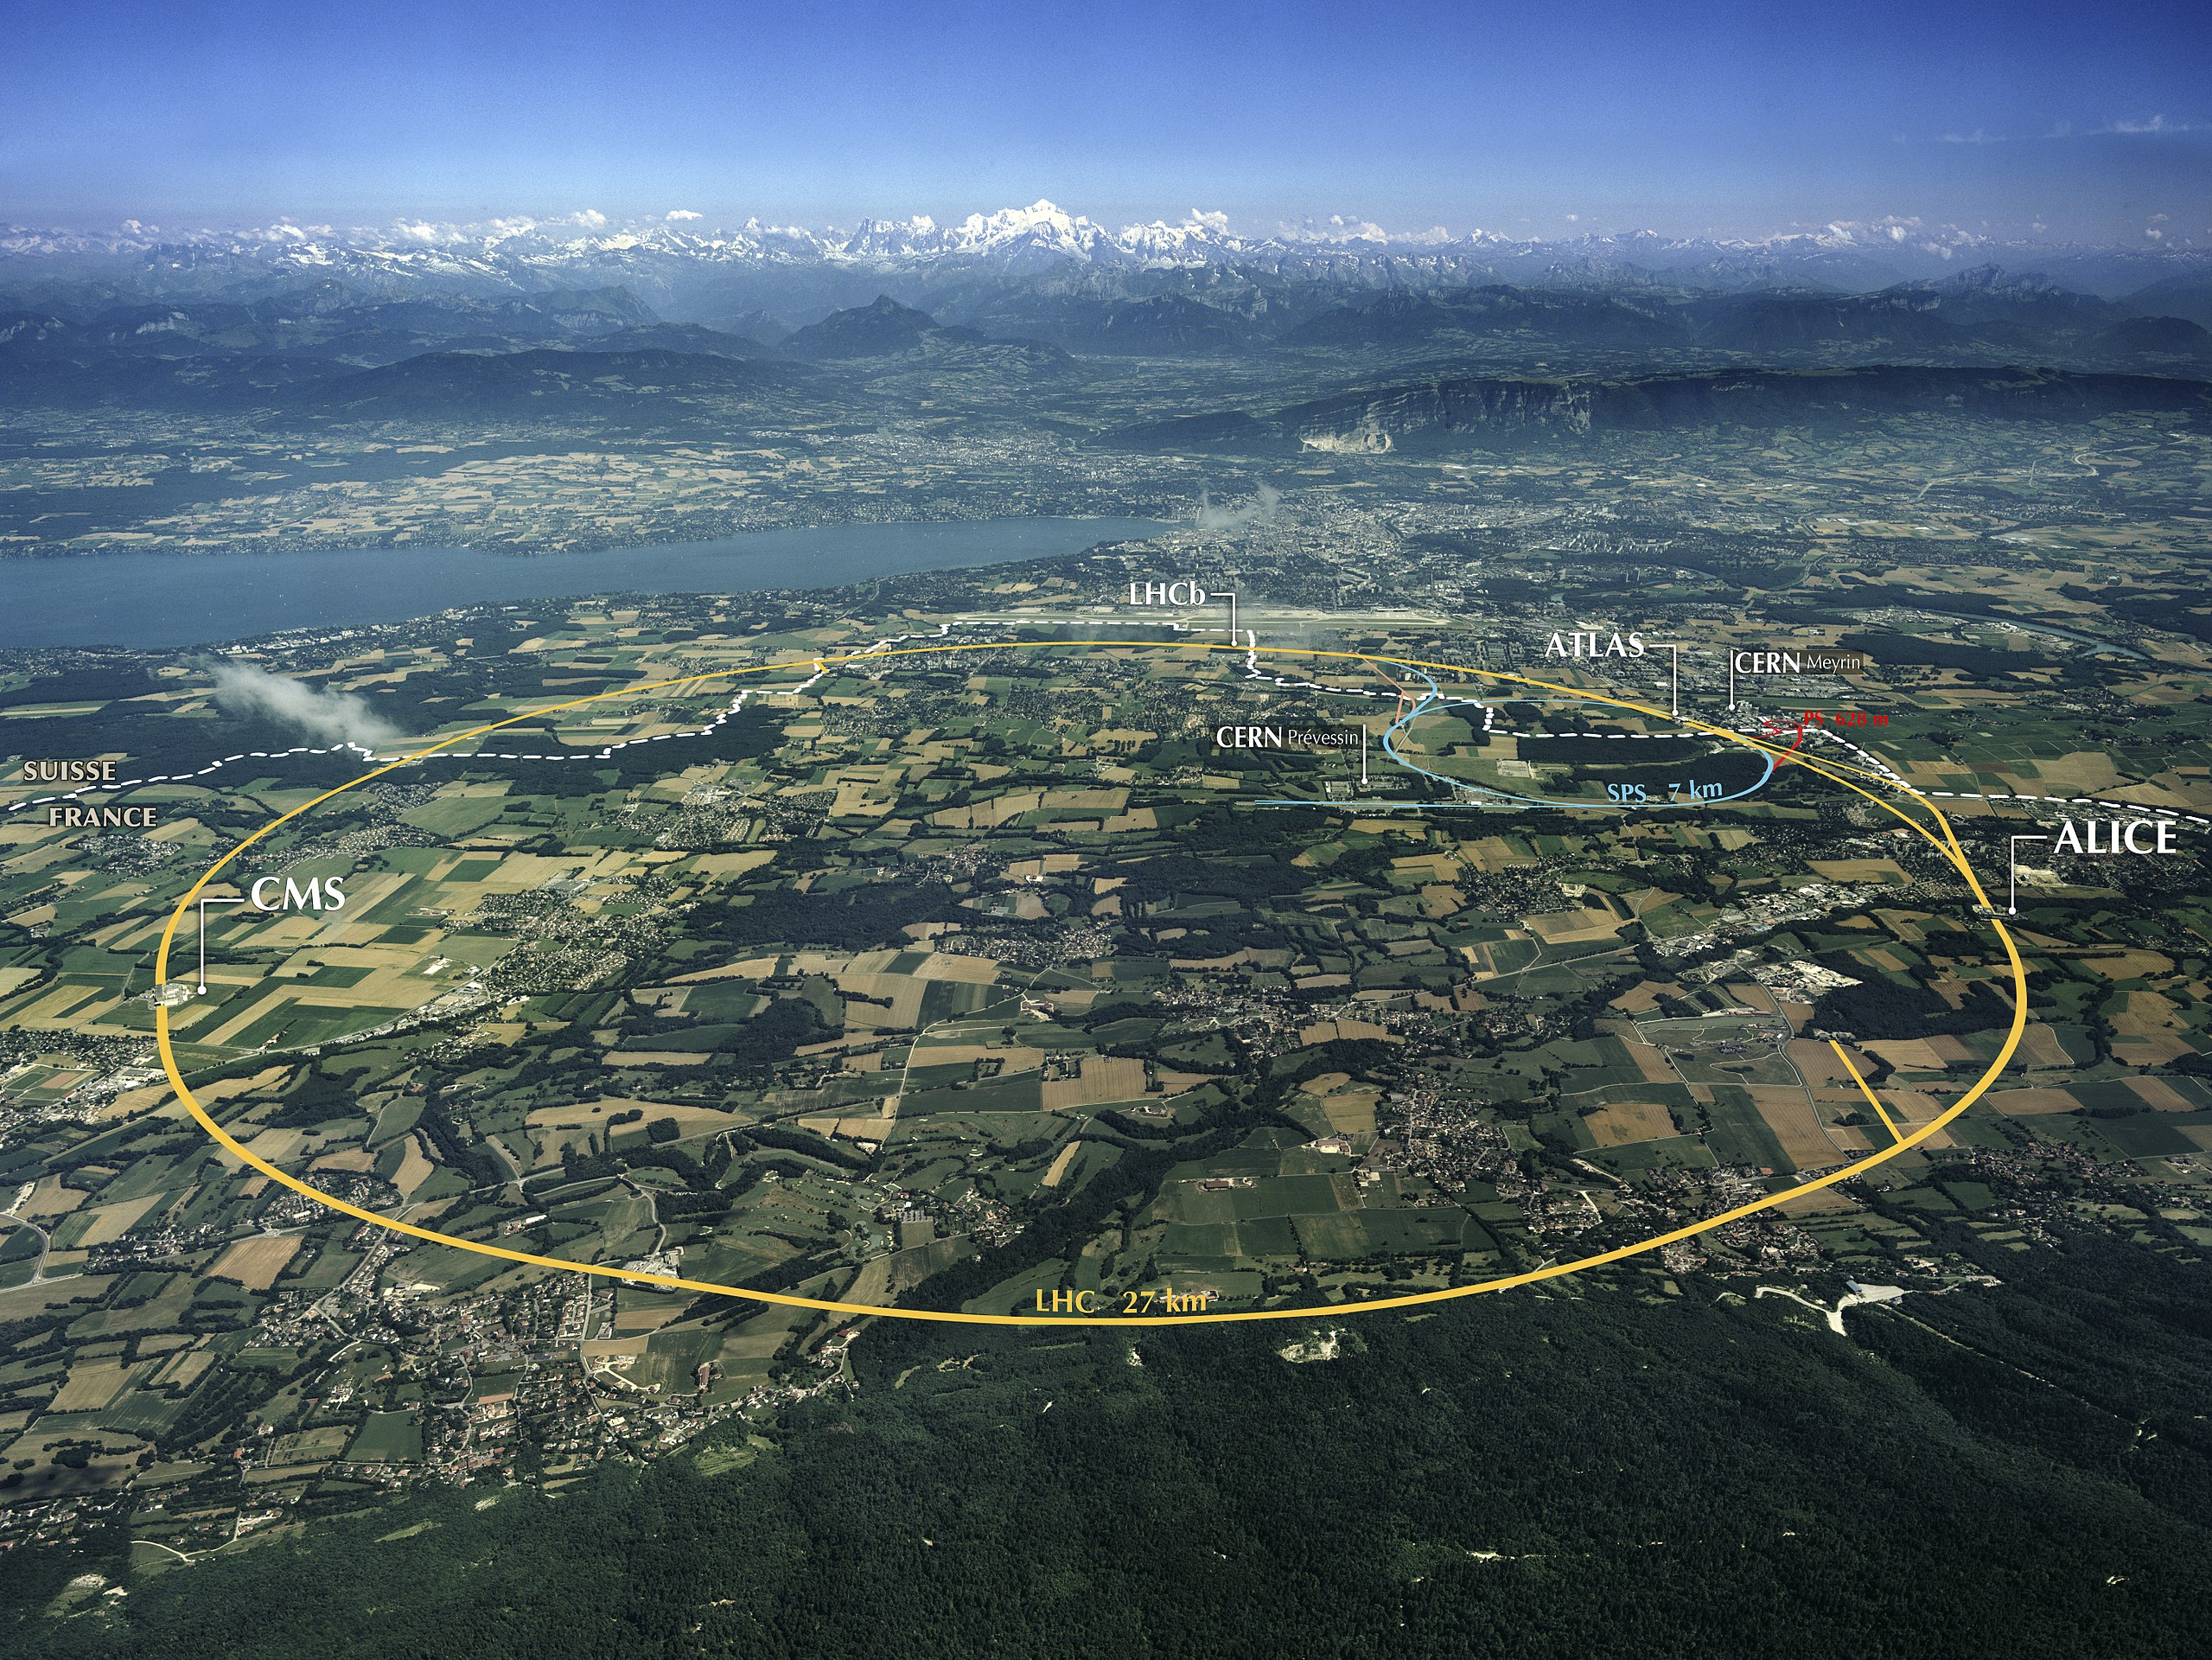
\includegraphics[width=0.45\textwidth,valign=c]{fig/lhc/cern_aerial_view.jpg}}
    \caption{
        A diagram illustrating the depth of the LHC beneath the surface (left), from Ref.~\cite{Servicegraphique:1708849}, and an aerial photograph of the entire CERN complex (right), from Ref.~\cite{Maximilien:1295244}. 
        The SPS and LHC tunnels illustrated in both figures. 
    }
    \label{fig:lhc_depth}
\end{figure}

\begin{figure}[htb]
    \centering
    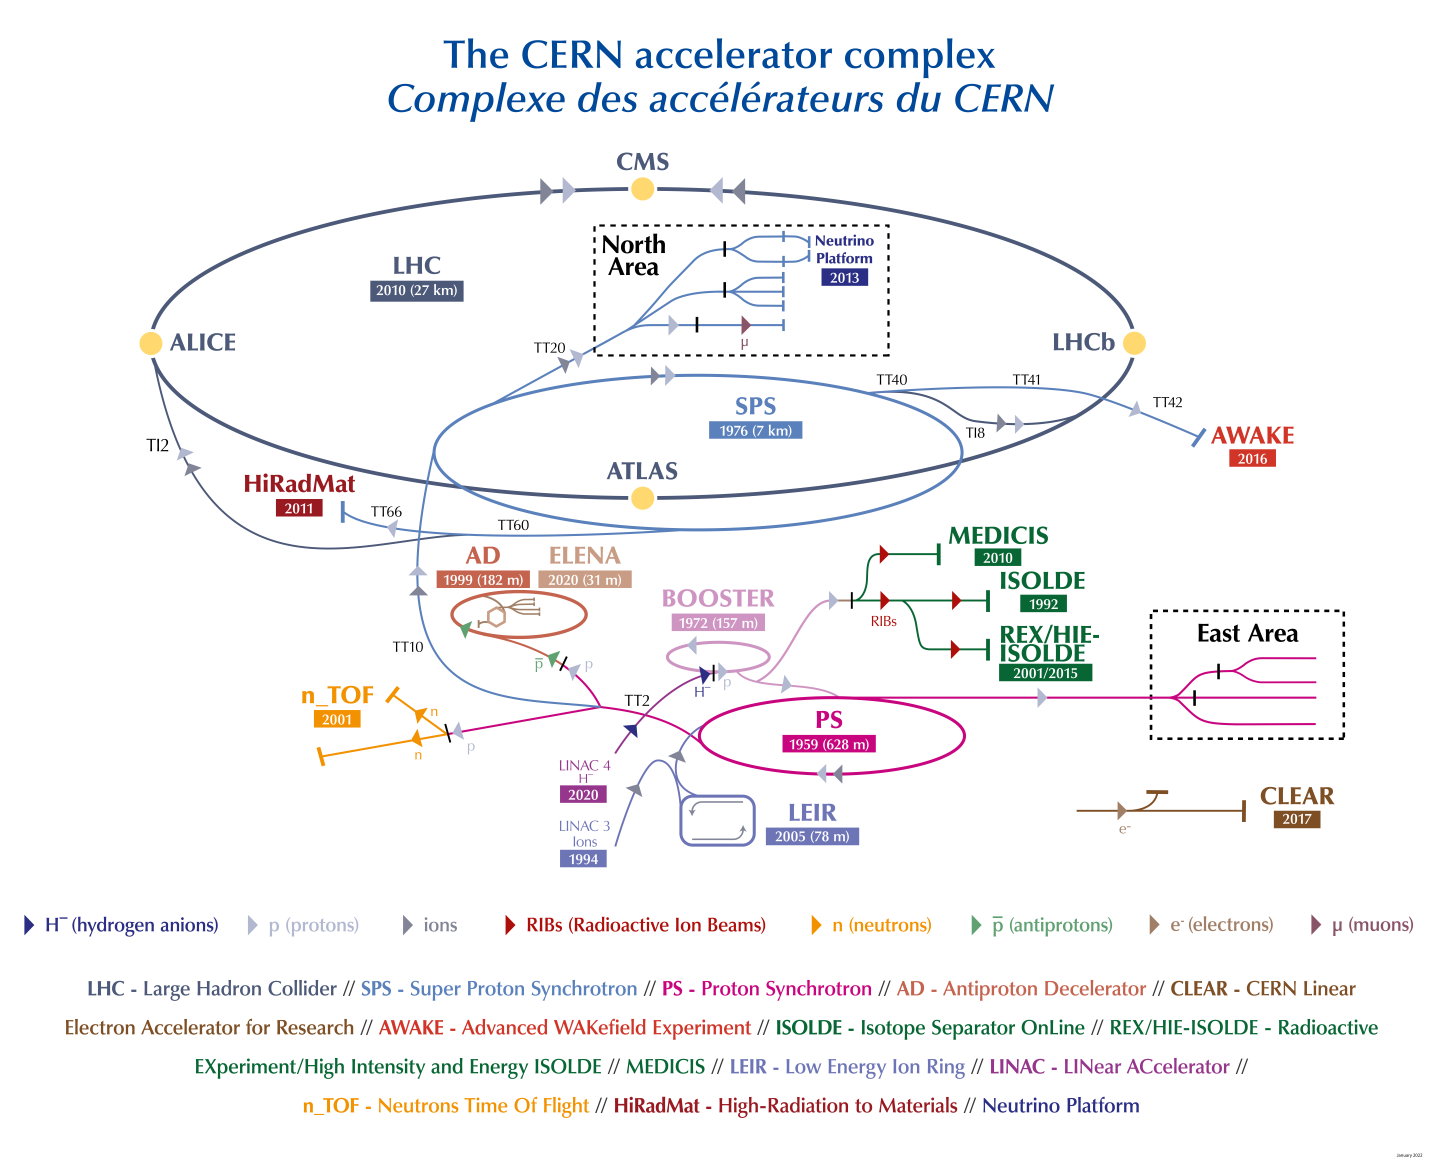
\includegraphics[width=0.95\textwidth]{fig/lhc/lhc_complex.png}
    \caption{
        The CERN complex illustrated in detail, from Ref.~\cite{Lopienska:2800984}. 
        The different stages of particle acceleration can be seen in detail, described here for protons. 
        First, negative hydrogen ions (H$^-$) generated by LINAC 4 are fed into BOOSTER, which strips the electrons from the H$^-$ ions, leaving only the protons, and accelerates them to 2\GeV. 
        Next, the Proton Synchrotron (PS) accelerates the protons to 26\GeV. 
        The PS feeds into the Super Proton Synchrotron (SPS) which further accelerates them to to 450\GeV. 
        Finally, the protons are fed into the LHC, which accelerates them to a final energy of 7\TeV. 
    }
    \label{fig:cern_complex}
\end{figure}

\begin{figure}[htb]
    \centering
    \subfloat{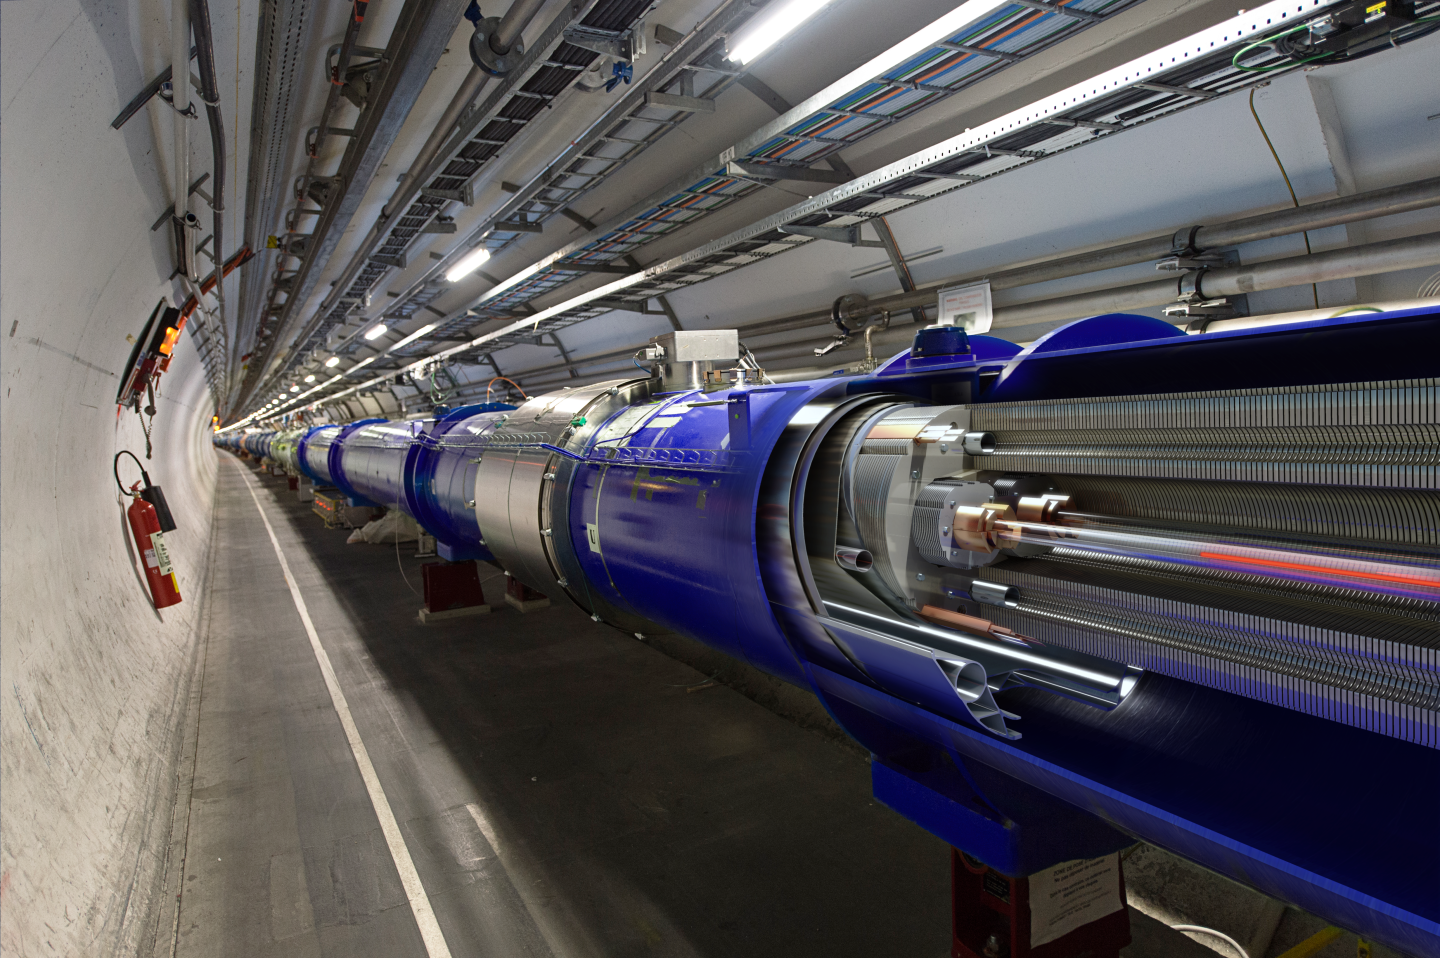
\includegraphics[width=0.475\textwidth,valign=c]{fig/lhc/dipole_cutaway.png}}\quad
    \subfloat{\includegraphics[width=0.425\textwidth,valign=c]{fig/lhc/dipole_jguiang.png}}
    \caption{
        A cutaway diagram illustrating the internals of a dipole magnet inside the LHC tunnel (left), from Ref.~\cite{Dominguez:1741036}, and a photograph of a decomissioned dipole magnet with a physicist for scale (right).
    }
    \label{fig:lhc_dipole}
\end{figure}

\clearpage

\section{The Compact Muon Solenoid}
The Compact Muon Solenoid (CMS) Experiment is one of two general purpose LHC experiments, the other being the ATLAS\footnotemark{} Experiment, among the four major experiments supported by the LHC~\cite{LHCWeb}, where the other two are more specialized: ALICE, for studying heavy ion collisons, and LHCb, for studying b quarks. 
\footnotetext{Whereas ATLAS is, putting it politely, a rather creative acronym: ``A Toroidal LHC ApparatuS.''}
Compared to ATLAS, which stands at a mighty $46\times25\times25$ meters in dimension, CMS is ``compact'' at a stout $21\times15\times15$ m, with a dedicated muon system and one of the world's largest solenoid magnets~\cite{ATLASWeb, CMSWeb}. 
See Fig.~\ref{fig:cms_labeled} for its exact specifications, and Figures~\ref{fig:cms_pics} and \ref{fig:cms_jguiang} for some beauty shots. 

\subsection{Overview}
CMS is composed of subdetectors arranged in concentric layers, where each layer interacts with, or completely absorbs, certain particles, producing an electric signal that can be used to measure some property of those particles. 
The innermost layer is the silicon tracker, which allows for the reconstruction of the trajectories of throughgoing charged particles (``tracks''). 
Next is the electromagnetic calorimeter (ECAL), which absorbs electrons and photons and records their individual energies. 
After the ECAL, there is the hadronic calorimeter (HCAL), which instead absorbs hadrons and records their individual energies. 
These first three layers---the tracker, ECAL, and HCAL---are surrounded by the superconducting solenoid, which immerses them in an approximately uniform magnetic field that runs parallel to the beamline. 
This is critical: because charged particles fly along curved trajectories in a magnetic field according to their charge and momentum, those properties can be inferred from a high-quality measurement of each particle's trajectory. 
Finally, there are alternating layers of muon chambers and iron support structures. 
The former, as the name suggests, detects throughgoing muons, which pass through all of the inner layers mostly unperturbed.
However, the latter is equally important: the iron ``return yoke'' guides the magnetic field outside of the solenoid, absorbs stray particles that make it past the inner layers, and supports the immense weight of CMS itself. 
In a perfect world, where the detector is 100\% efficient, the exact identity of any individual particle can be inferred based on which detectors registered a signal (Fig.~\ref{fig:cms_particle_id}). 
For example, a photon only leaves a deposit in the ECAL, while a charged hadron leaves behind ``hits'' in the tracker as well as a deposit in the HCAL. 
The exact function of each subdetector layer described here is detailed below.

\begin{figure}[htb]
    \centering
    \includegraphics[width=0.9\textwidth]{fig/cms/cms_labeled.jpg}
    \caption{
        A detailed cutaway diagram of CMS, with each subdetector labeled with its name and some its characteristics. 
    }
    \label{fig:cms_labeled}
\end{figure}

\begin{figure}[htb]
    \centering
    \subfloat{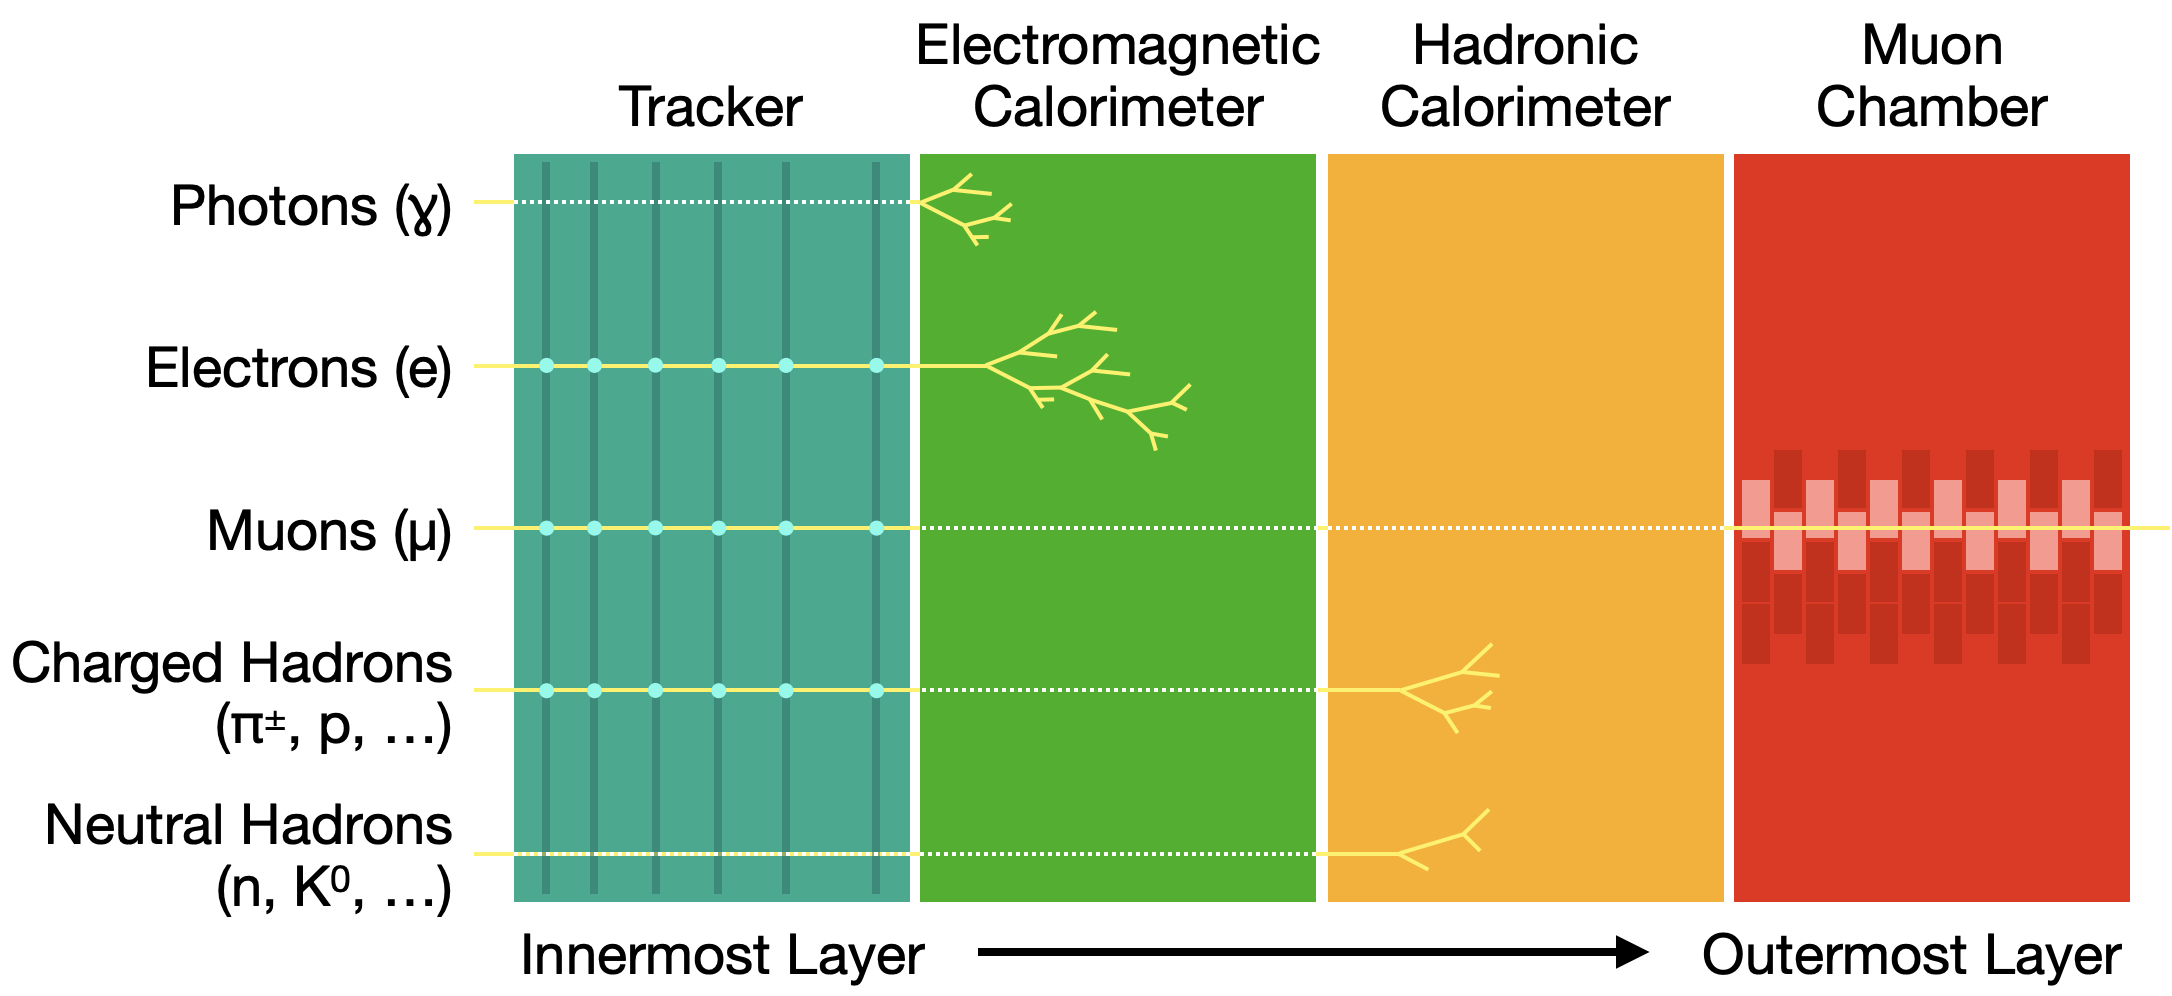
\includegraphics[width=0.465\textwidth,valign=c]{fig/cms/particle_id_sandwich.png}}\quad
    \subfloat{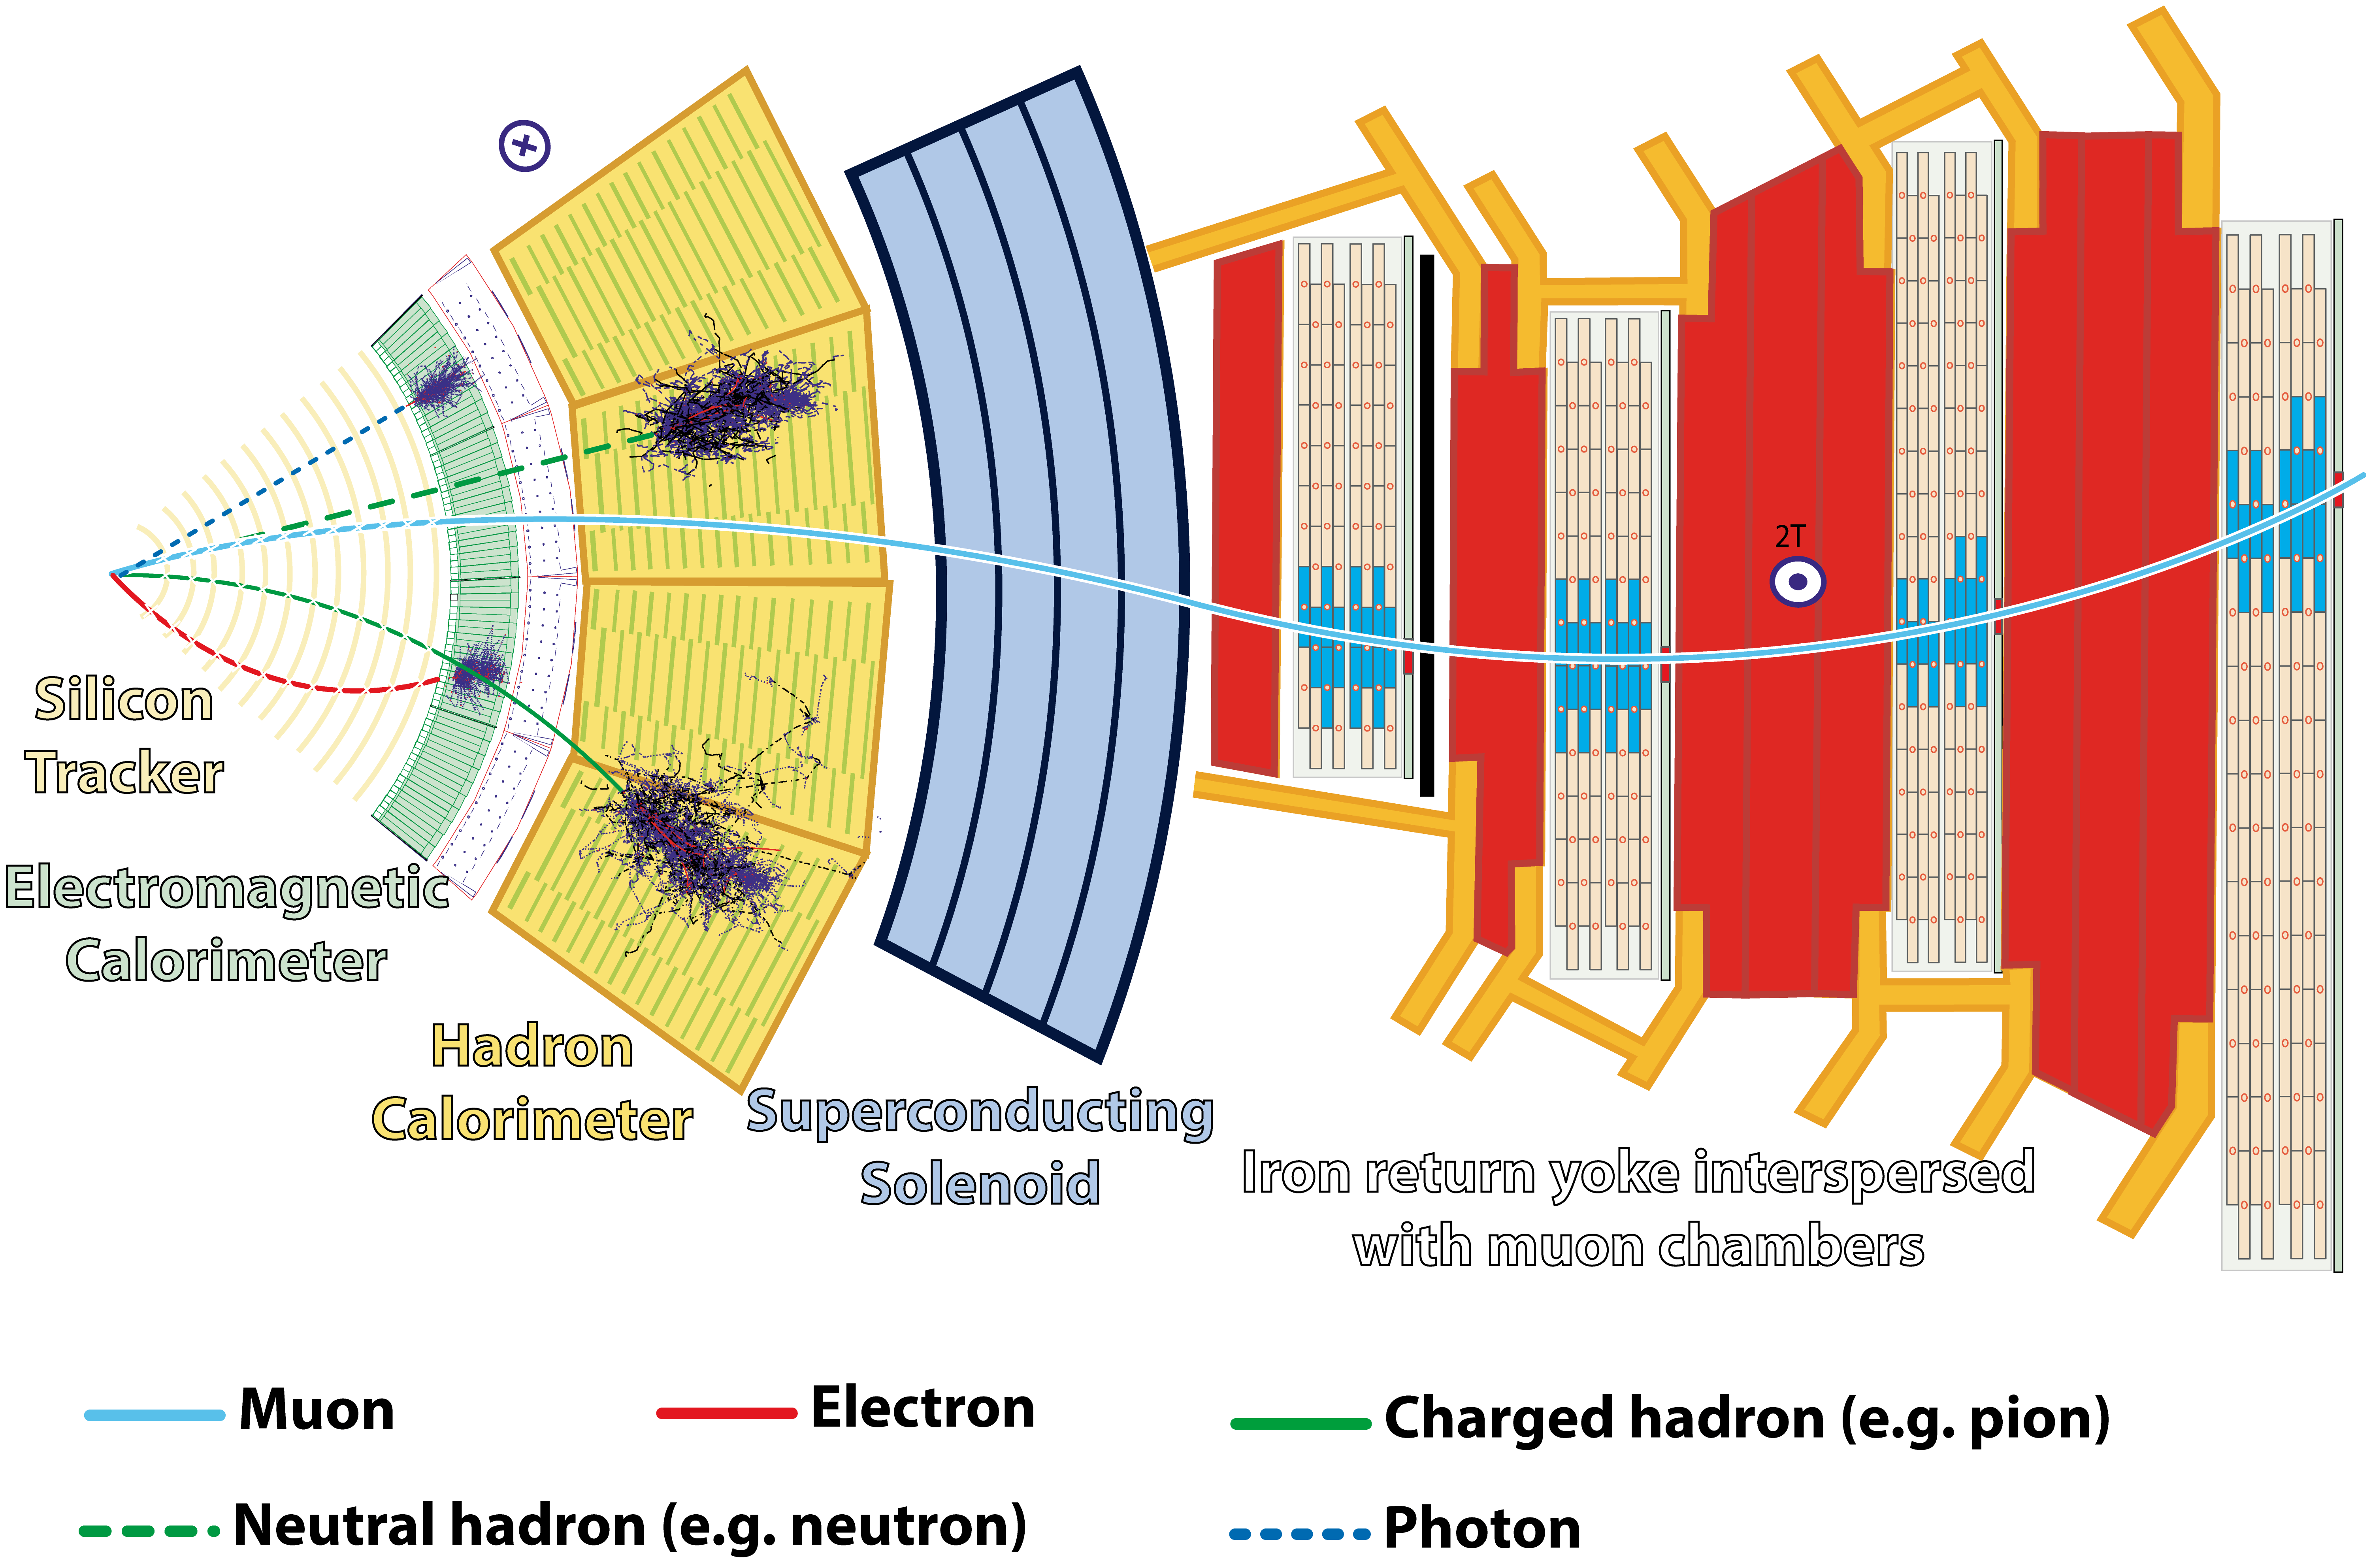
\includegraphics[width=0.435\textwidth,valign=c]{fig/cms/cms_slice.png}}
    \caption{
        A generic, general-purpose particle detector (left) and a transverse slice of CMS (right), from Ref.~\cite{Barney:2120661}, showing the signals left by different kinds of particles.
    }
    \label{fig:cms_particle_id}
\end{figure}

\subsection{Superconducting solenoid}
The curve of a track is critical, as it allows us to infer the charge and momentum of a particle. 
However, in a weak magnetic field, the particles produced at the LHC would have nearly straight tracks, due to the large proton-proton collision energy. 
The magnetic field inside of CMS must therefore be very large. 
It should also be nearly uniform everywhere in order to make the computation of each particle's charge and momentum as simple as possible. 
The CMS magnet must also be large in dimension, however, as it must surround the tracker, ECAL, and HCAL, since it would otherwise block outgoing particles. 

By winding copper wire into a helix and passing a current through it, we can generate an magnetic field whose strength is directly proportional to the current and number of turns of the wire, but inversely proportional to the length of the helix. 
Within the volume of the helix, the magnetic field will be almost uniformly oriented in a single direction, determined by the orientation of the helix and direction of the current (Fig.~\ref{fig:cms_magnet_ideal}). 
This is not true outside of the helix where the magnetic field lines curve in space. 

The CMS magnet~\cite{CERN-LHCC-97-010} is a massive realization of a solenoid. 
It is comprised of over 2000 turns of Rutherford wire, which has a rectangular cross section (Fig.~\ref{fig:cms_magnet}). 
In operation, it is cooled to superconducting temperatures, such that a high current of 20 kiloamperes\footnotemark{} can be passed through the coil without destroying it. 
\footnotetext{For scale, this is $100\,000$ times larger than the minimum fatal current for humans (100--200 milliamperes)~\cite{10.1093/ptj/46.9.968}.}
This configuration allows the CMS magnet to produce a mostly uniform magnetic field of 4 T inside of the solenoid volume. 
That is 2--4 times larger than an MRI, which are typically 0.5--1.5 T~\cite{Berger2002-gs}, within a volume that is 1000 times larger. % TODO: citation needed for volume of an MRI?
Outside of the solenoid volume, however, we still want a fairly uniform magnetic field in order to maintain good momentum resolution for muons. 
To achieve this, the iron support structures that hold CMS together are also designed to guide the magnetic field lines (Fig.~\ref{fig:cms_magnet_field}). 
Inside of the iron, the magnetic field runs uniformly parallel to the field inside of the solenoid, but in the opposite direction---this gives muon tracks a characteristic S-shape in the transverse plane. 

\begin{figure}[htb]
    \centering
    \subfloat[]{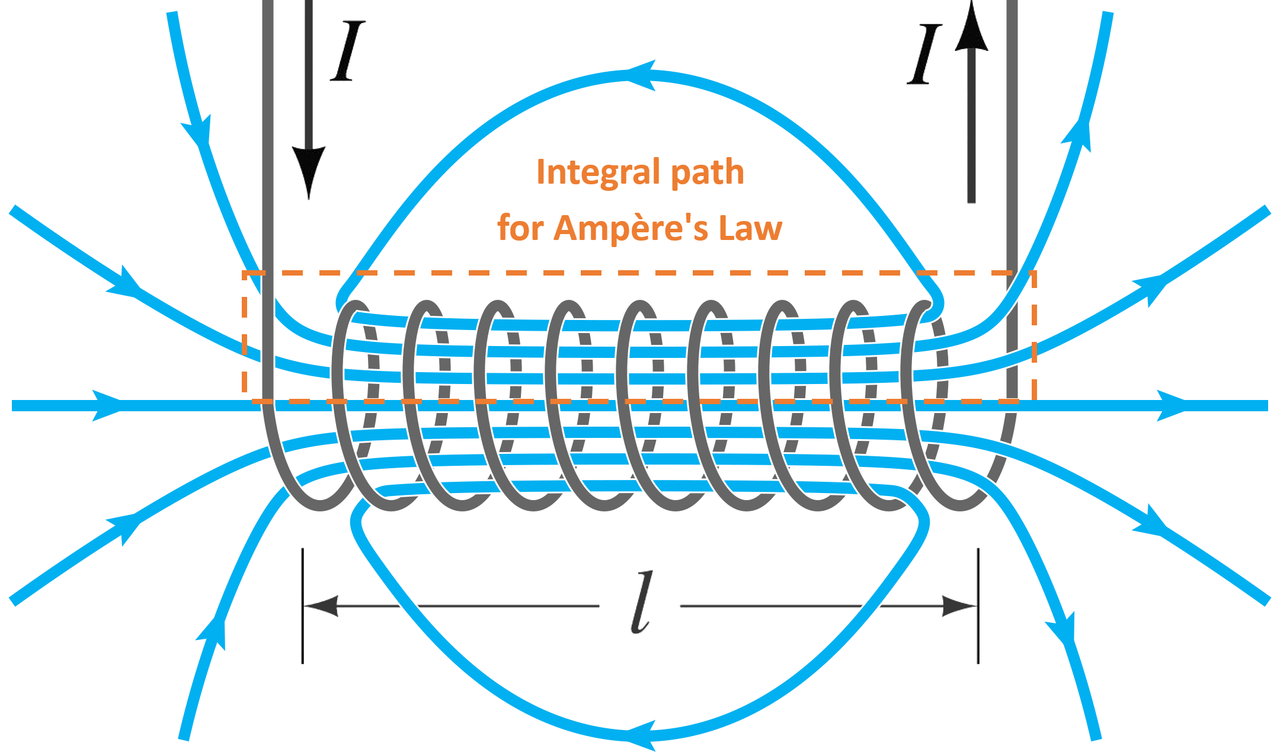
\includegraphics[width=0.4\textwidth,valign=c]{fig/cms/solenoid_ideal.png}\label{fig:cms_magnet_ideal}}\quad
    \subfloat[]{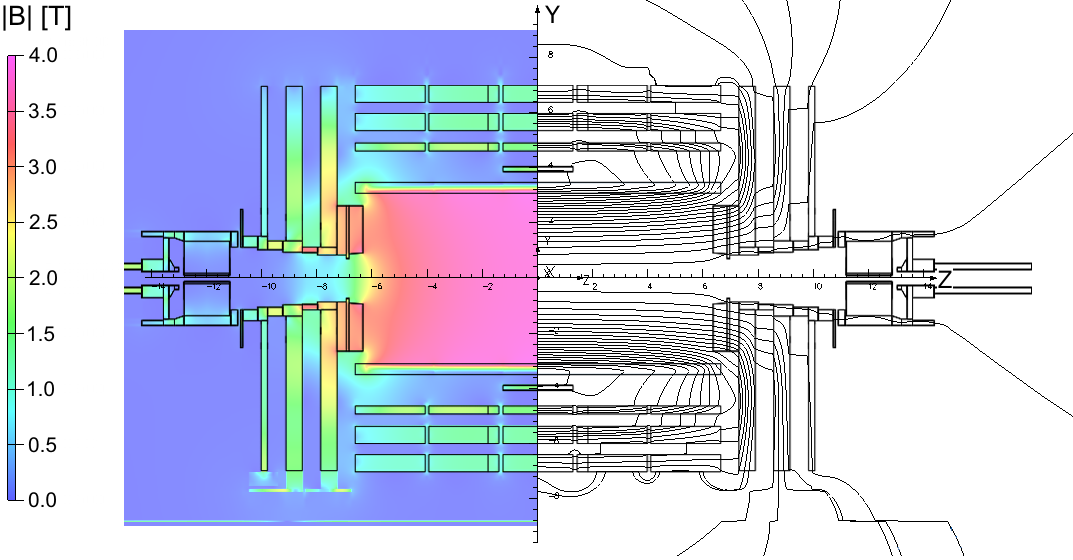
\includegraphics[width=0.5\textwidth,valign=c]{fig/cms/solenoid_field.png}\label{fig:cms_magnet_field}}
    \caption{
        The field lines of an ideal solenoid (a) and those of the CMS magnet (b), from Ref.~\cite{CMS:2009moq}. 
        For the ideal solenoid, the magnetic field is described by a simple equation: $B = \mu_0\frac{NI}{l}$, where $\mu_0$ is the magnetic constant, $N$ is the number of turns, $I$ is the current, and $l$ is the length of the helix. 
    }
    \label{fig:cms_fields}
\end{figure}

\begin{figure}[htb]
    \centering
    \subfloat{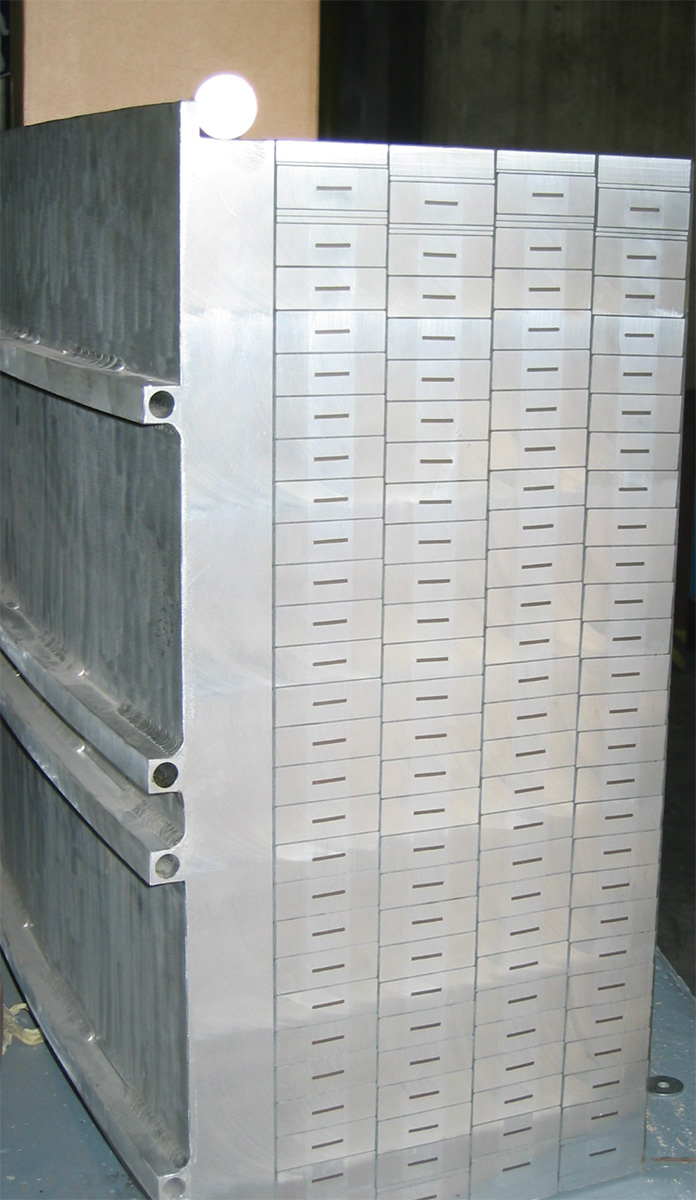
\includegraphics[width=0.3\textwidth,valign=c]{fig/cms/solenoid_section.jpg}}\quad
    \subfloat{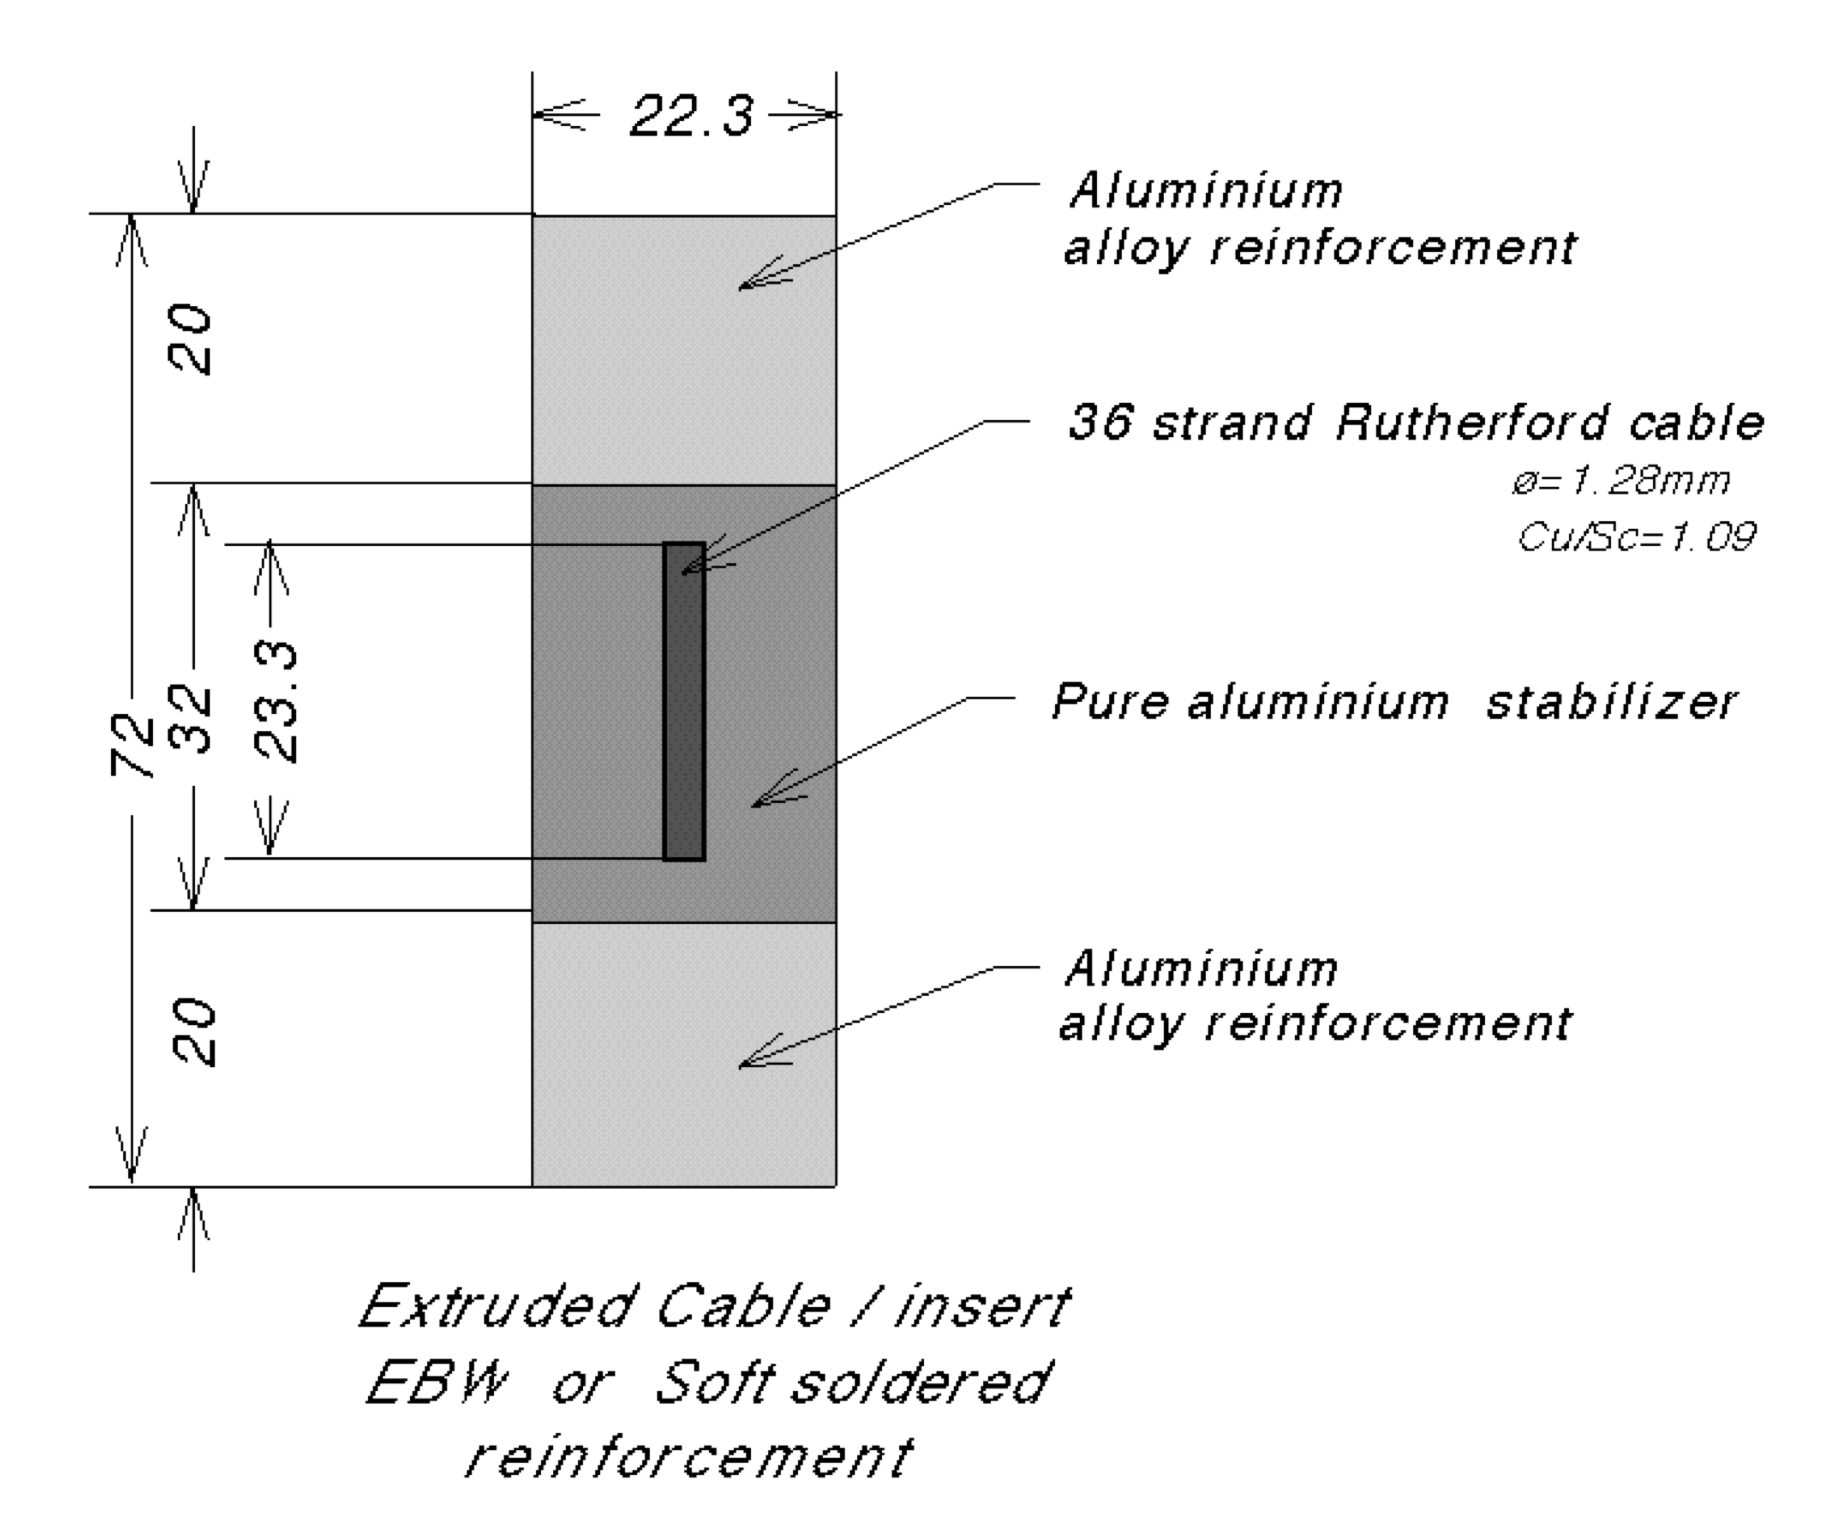
\includegraphics[width=0.6\textwidth,valign=c]{fig/cms/solenoid_cable.png}}
    \caption{
        A photograph of a section of the CMS magnet, from Ref.~\cite{CourierSolenoid}, showing the cross section of the solenoid windings (left), and a diagram of a single winding, from Ref.~\cite{CERN-LHCC-97-010} (right). 
    }
    \label{fig:cms_magnet}
\end{figure}

\subsection{Silicon tracker}

\begin{figure}[htb]
    \centering
    \subfloat{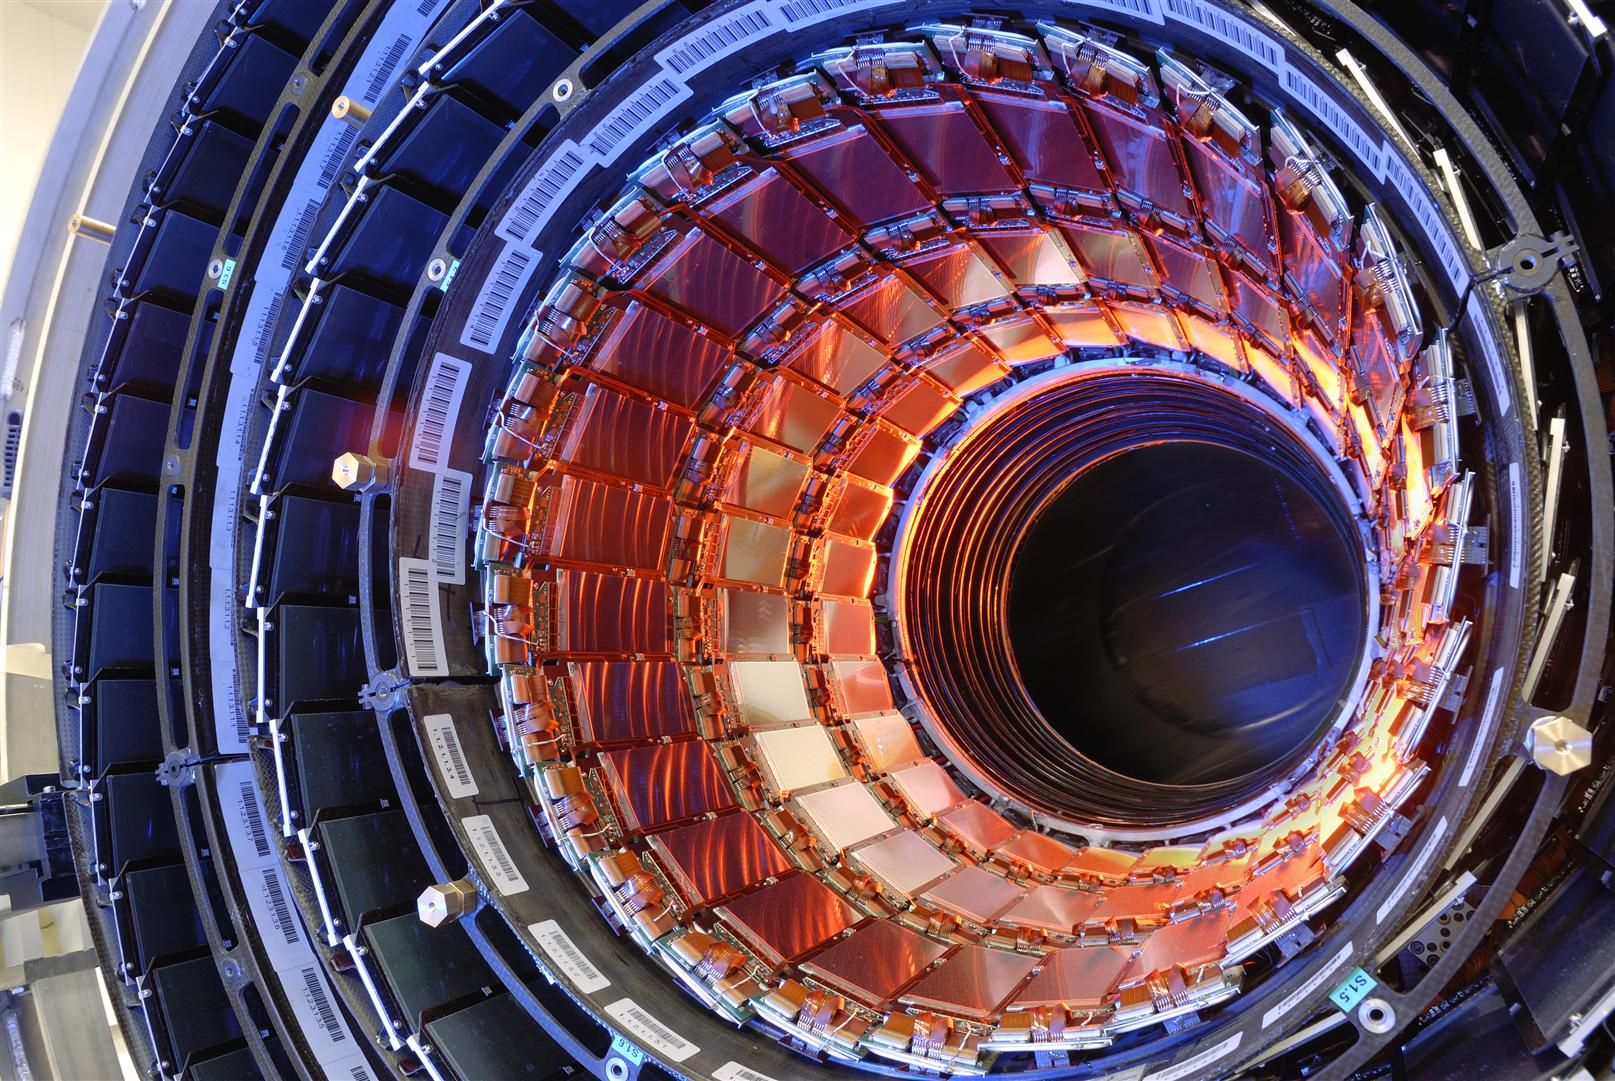
\includegraphics[width=0.465\textwidth,valign=c]{fig/cms/tracker_rainbow.jpg}}\quad
    \subfloat{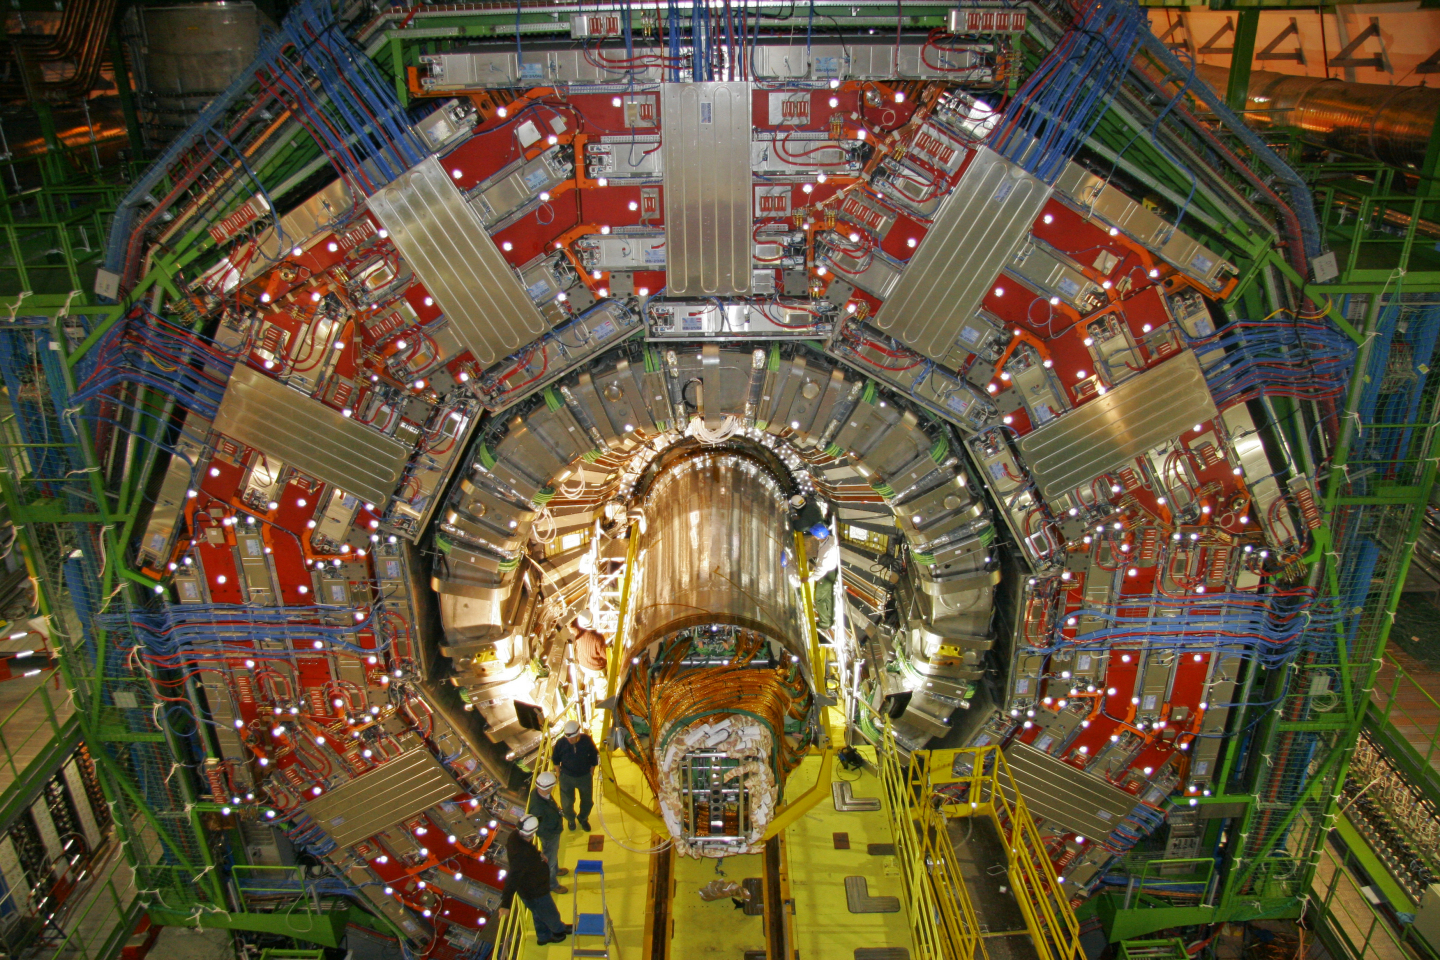
\includegraphics[width=0.435\textwidth,valign=c]{fig/cms/tracker_install.jpg}}
    \caption{
        A photograph of the CMS outer tracker (left), from Ref.~\cite{Maximilien:995912}, and the installation of the entire tracker (right), from Ref~\cite{Hoch:1275108}. 
    }
    \label{fig:cms_tracker}
\end{figure}

\subsection{Electromagnetic calorimeter}

\begin{figure}[htb]
    \centering
    \subfloat{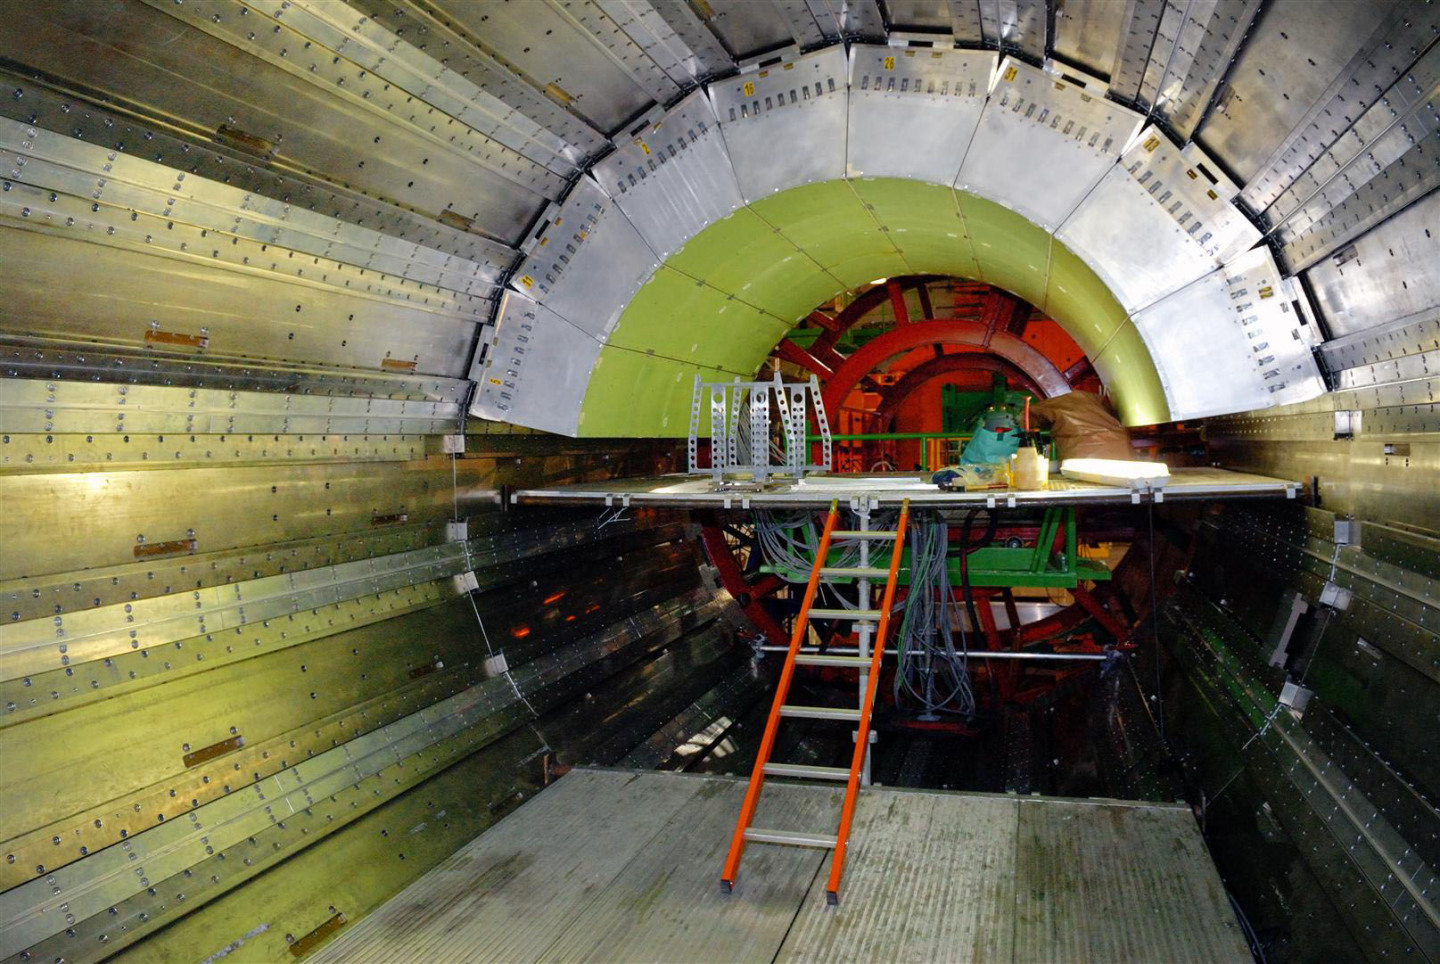
\includegraphics[width=0.465\textwidth,valign=c]{fig/cms/ecal_installed.jpg}}\quad
    \subfloat{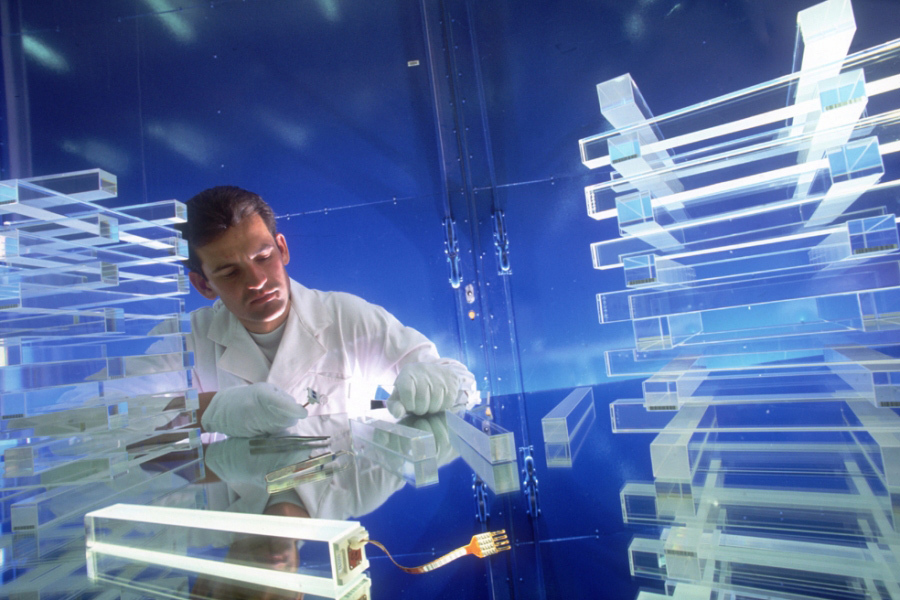
\includegraphics[width=0.435\textwidth,valign=c]{fig/cms/ecal_crystals.jpg}}
    \caption{
        A photograph of the CMS electromagnetic calorimeter (ECAL) after half of the modules had been installed (left) and physicist Lucas Taylor posed with the lead tungstade scintillator crystals used in the ECAL (right). 
        Both photographs are from Ref.~\cite{Brice:1431477}.
    }
    \label{fig:cms_ecal}
\end{figure}

\subsection{Hadronic calorimeter}

\begin{figure}[htb]
    \centering
    \subfloat{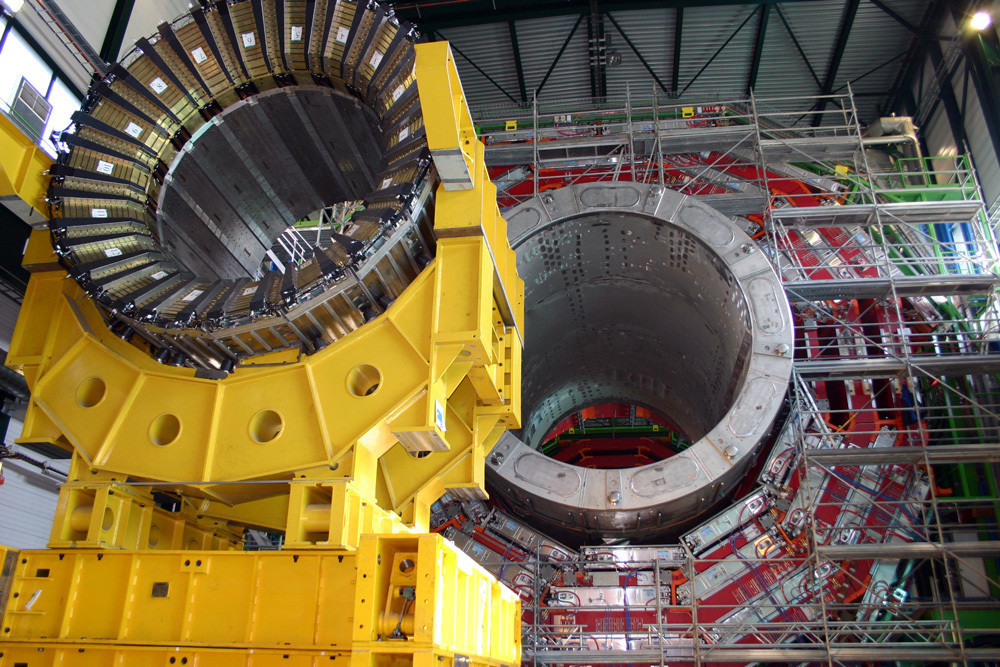
\includegraphics[width=0.465\textwidth,valign=c]{fig/cms/hcal_removed.jpg}}\quad
    \subfloat{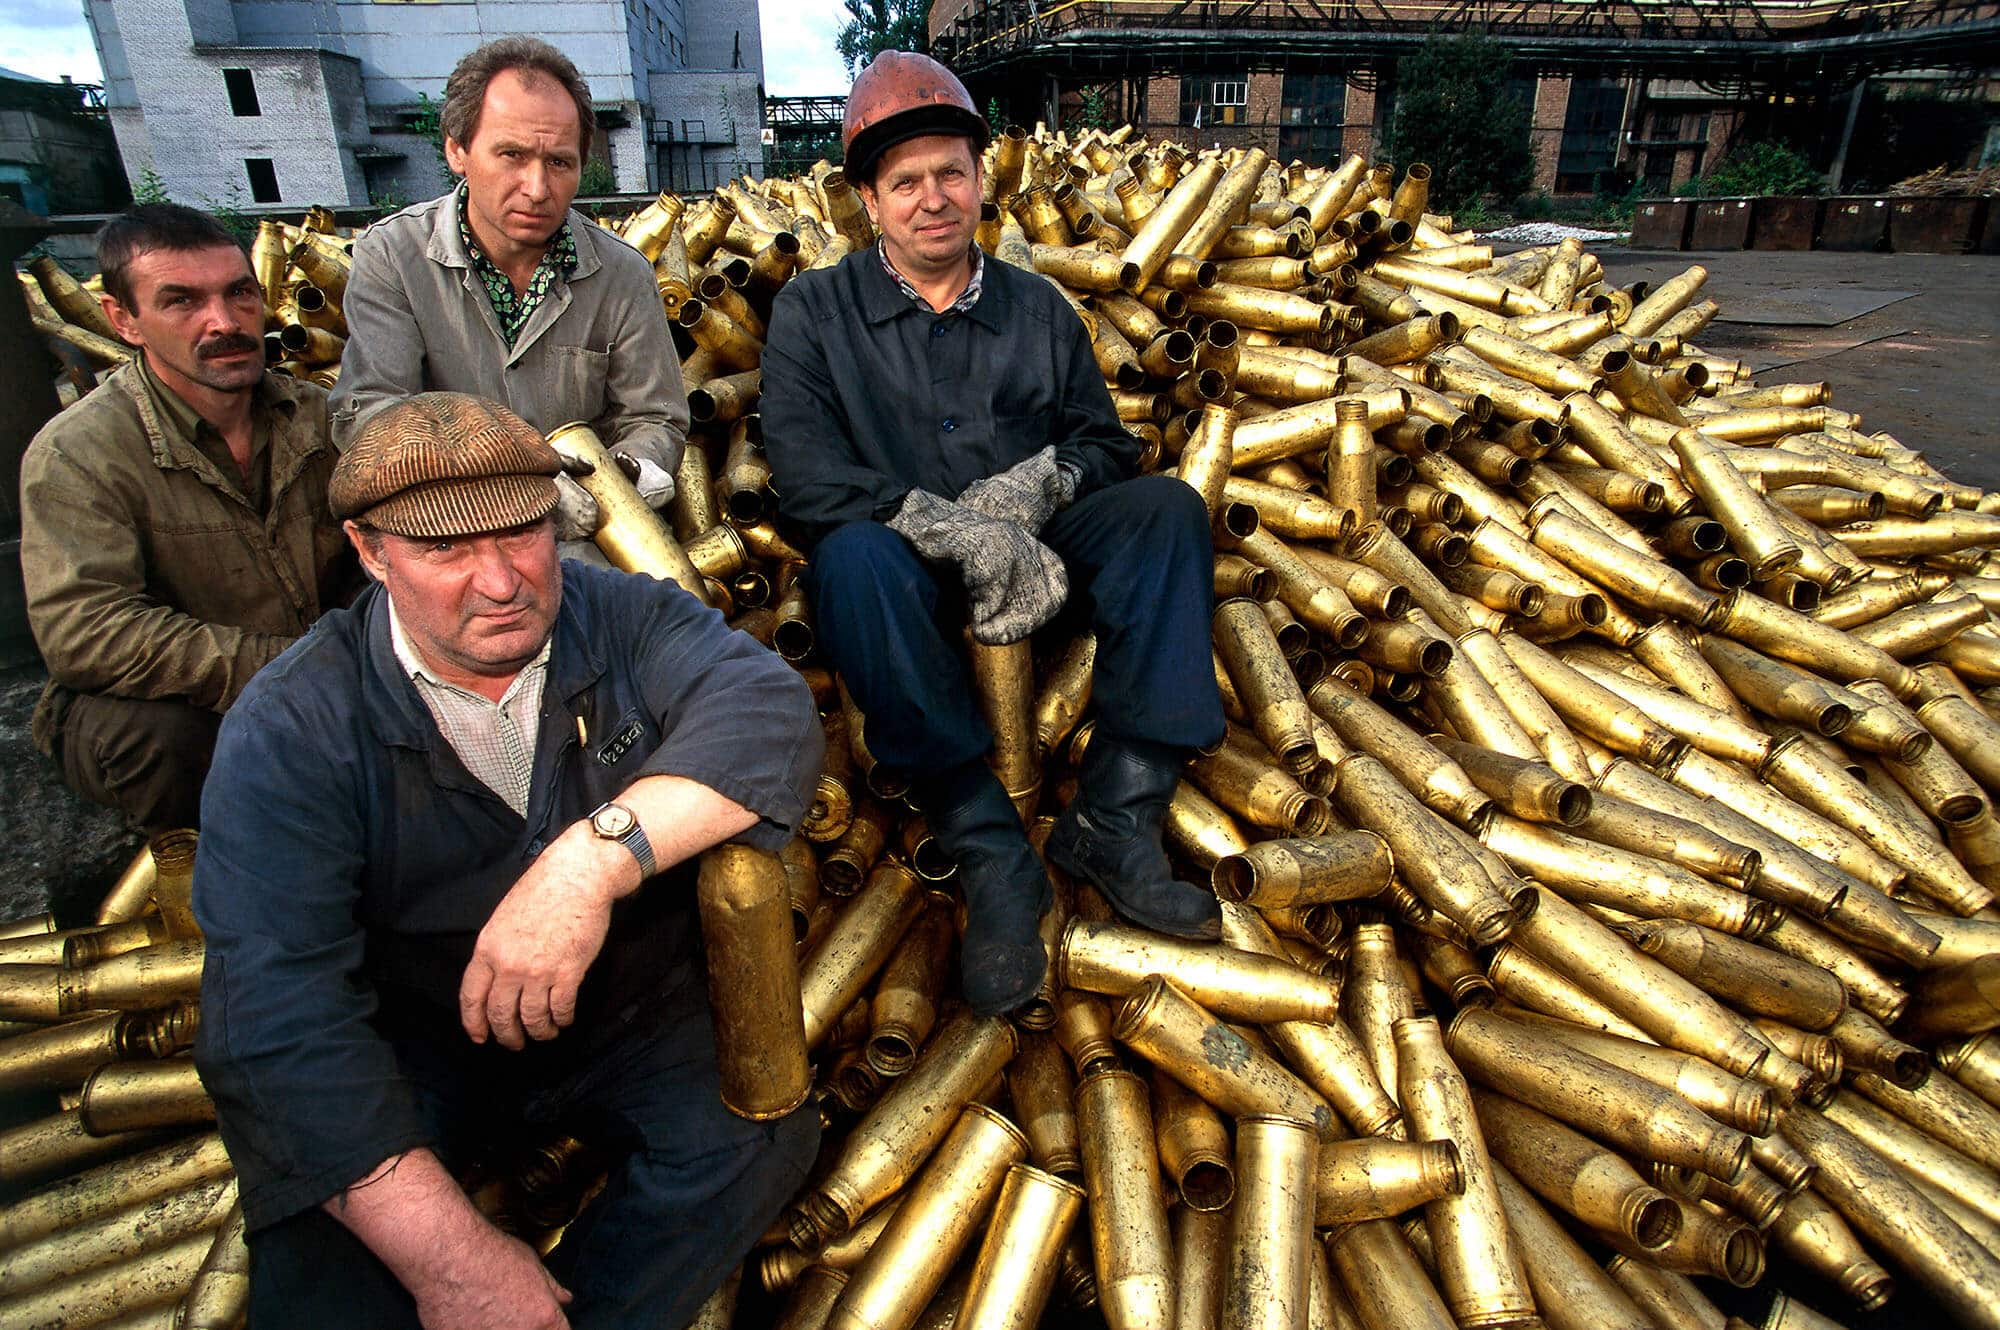
\includegraphics[width=0.435\textwidth,valign=c]{fig/cms/hcal_russian.jpg}}
    \caption{
        A photograph of the CMS hadronic calorimeter (HCAL) in front of the magnet and muon chambers before the detector was installed in the experiment cavern (left), from Ref.~\cite{Brice:1431485}, and workers in Mormansk sitting on the decomissioned WWII artillery shells used to supply the brass for the HCAL (right), from Ref.~\cite{GinterRussianDudes}.
    }
    \label{fig:cms_hcal}
\end{figure}

\subsection{Muon chambers}

\begin{figure}[htb]
    \centering
    \subfloat{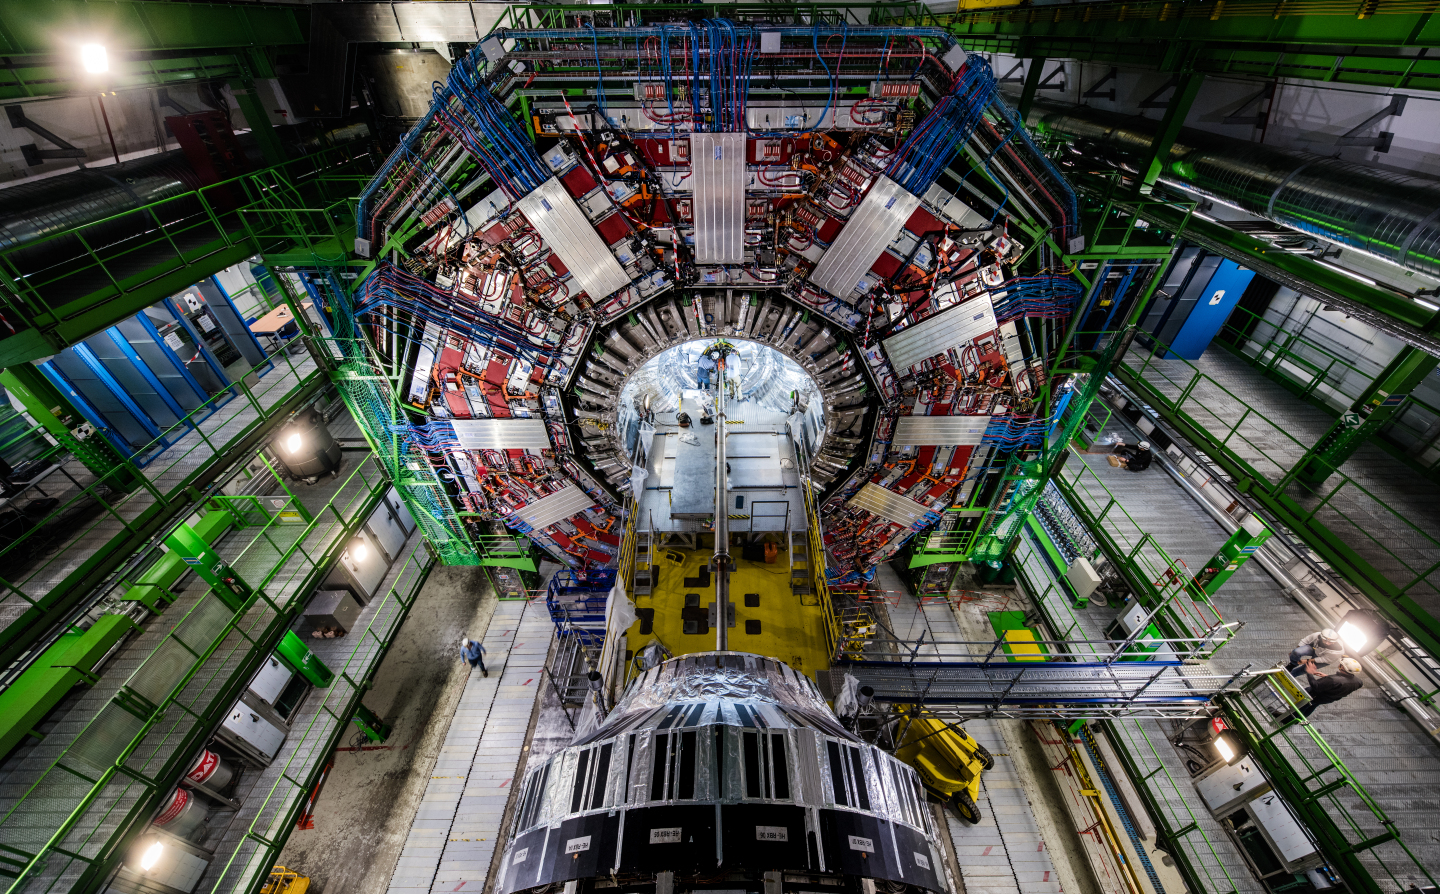
\includegraphics[width=0.465\textwidth]{fig/cms/cms_picture1.jpg}}\quad
    \subfloat{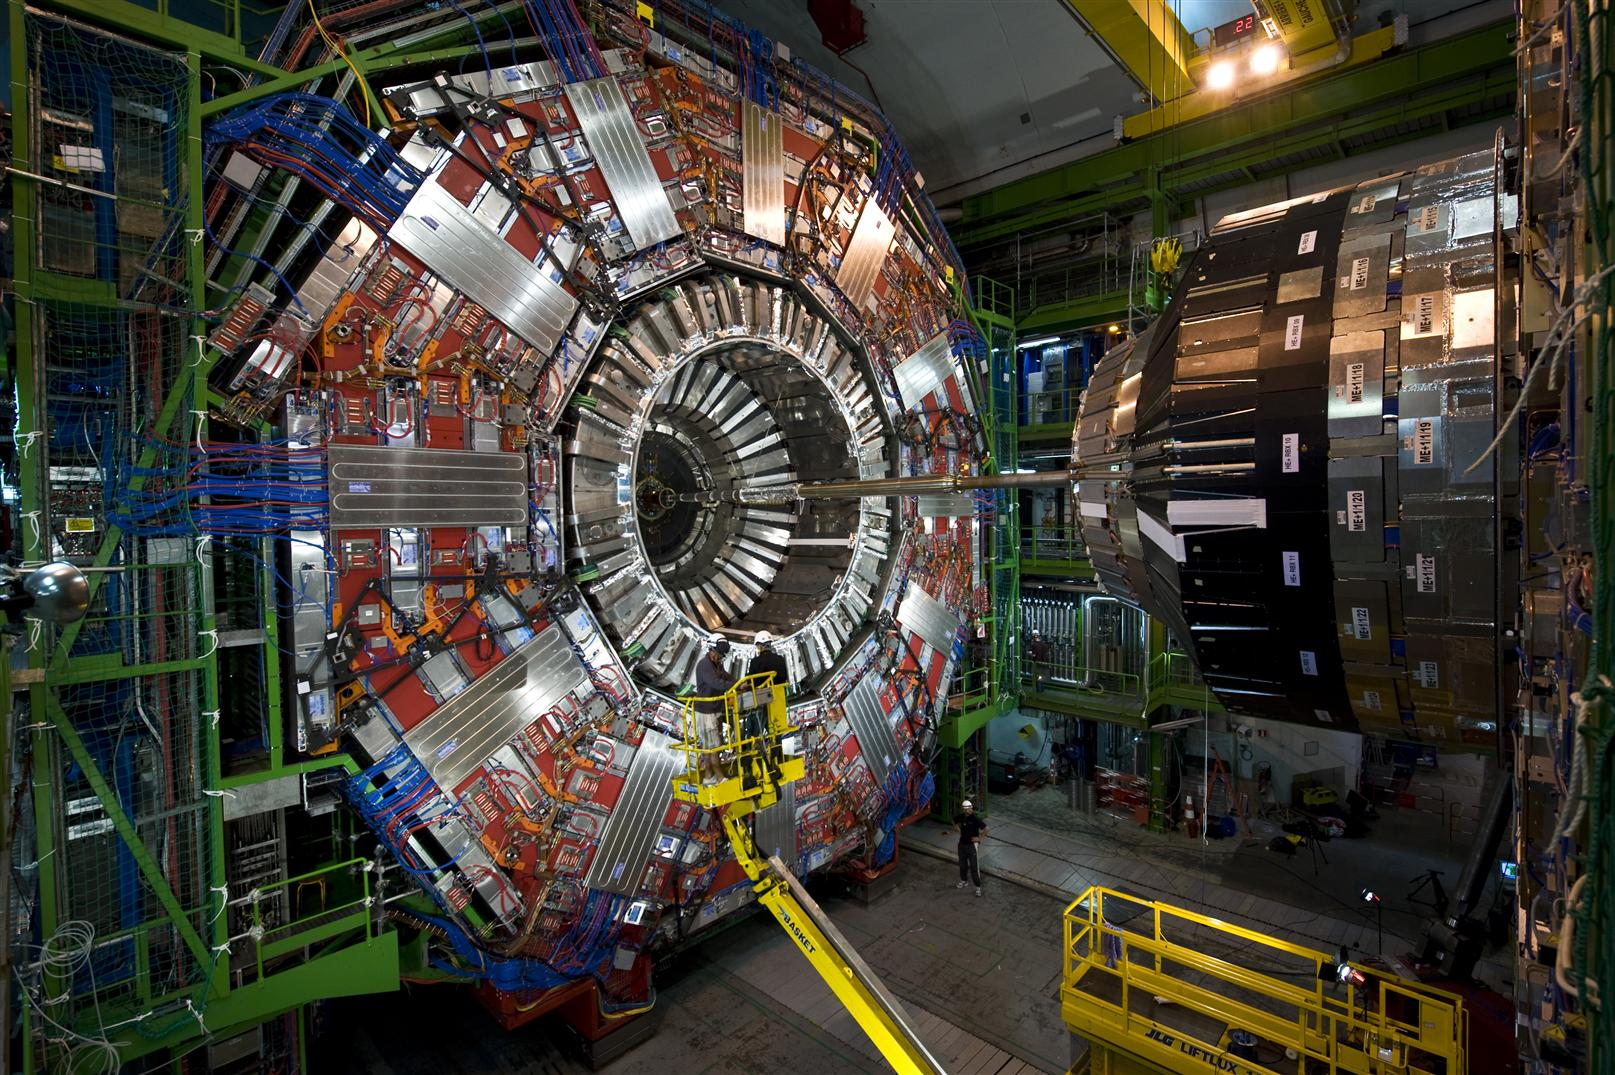
\includegraphics[width=0.435\textwidth]{fig/cms/cms_picture2.jpg}}
    \caption{
        The Compact Muon Solenoid in all of its glory, with one of the endcaps separated from the main body of the experiment, pictured from the top (left) and side (right). 
    }
    \label{fig:cms_pics}
\end{figure}

\begin{figure}[htb]
    \centering
    \subfloat{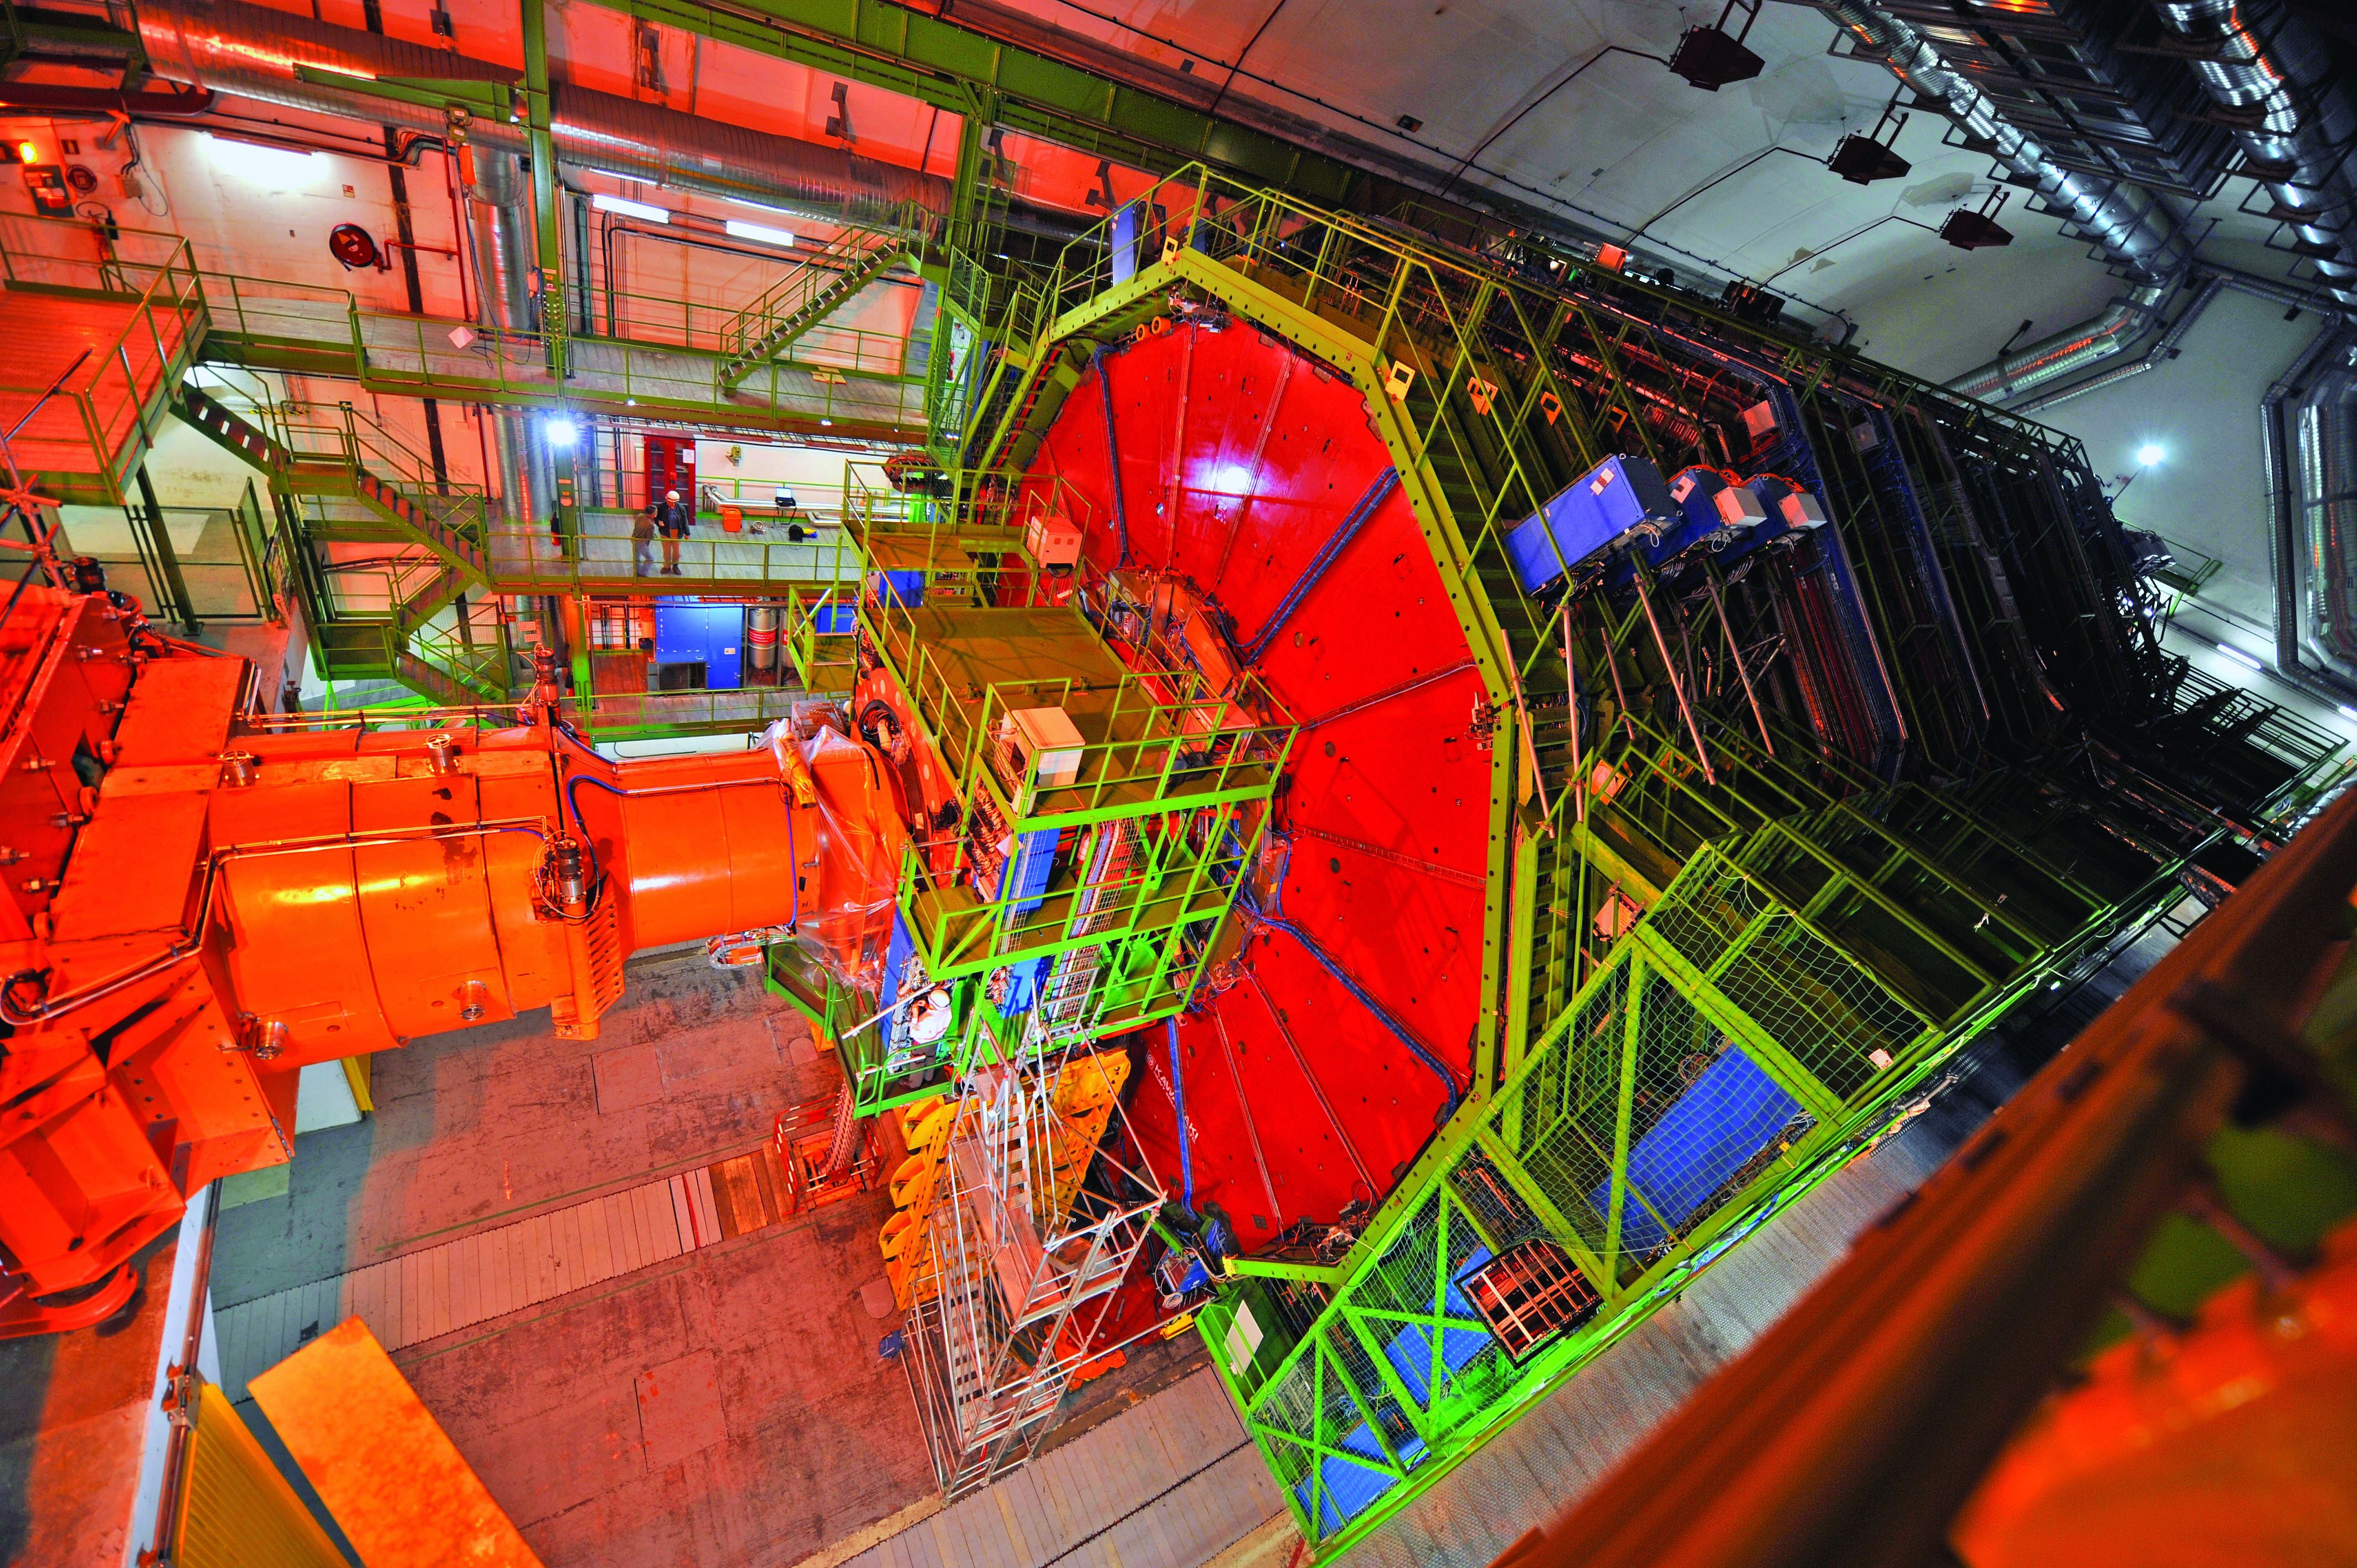
\includegraphics[width=0.482\textwidth,valign=c]{fig/cms/cms_picture3.jpg}}\quad
    \subfloat{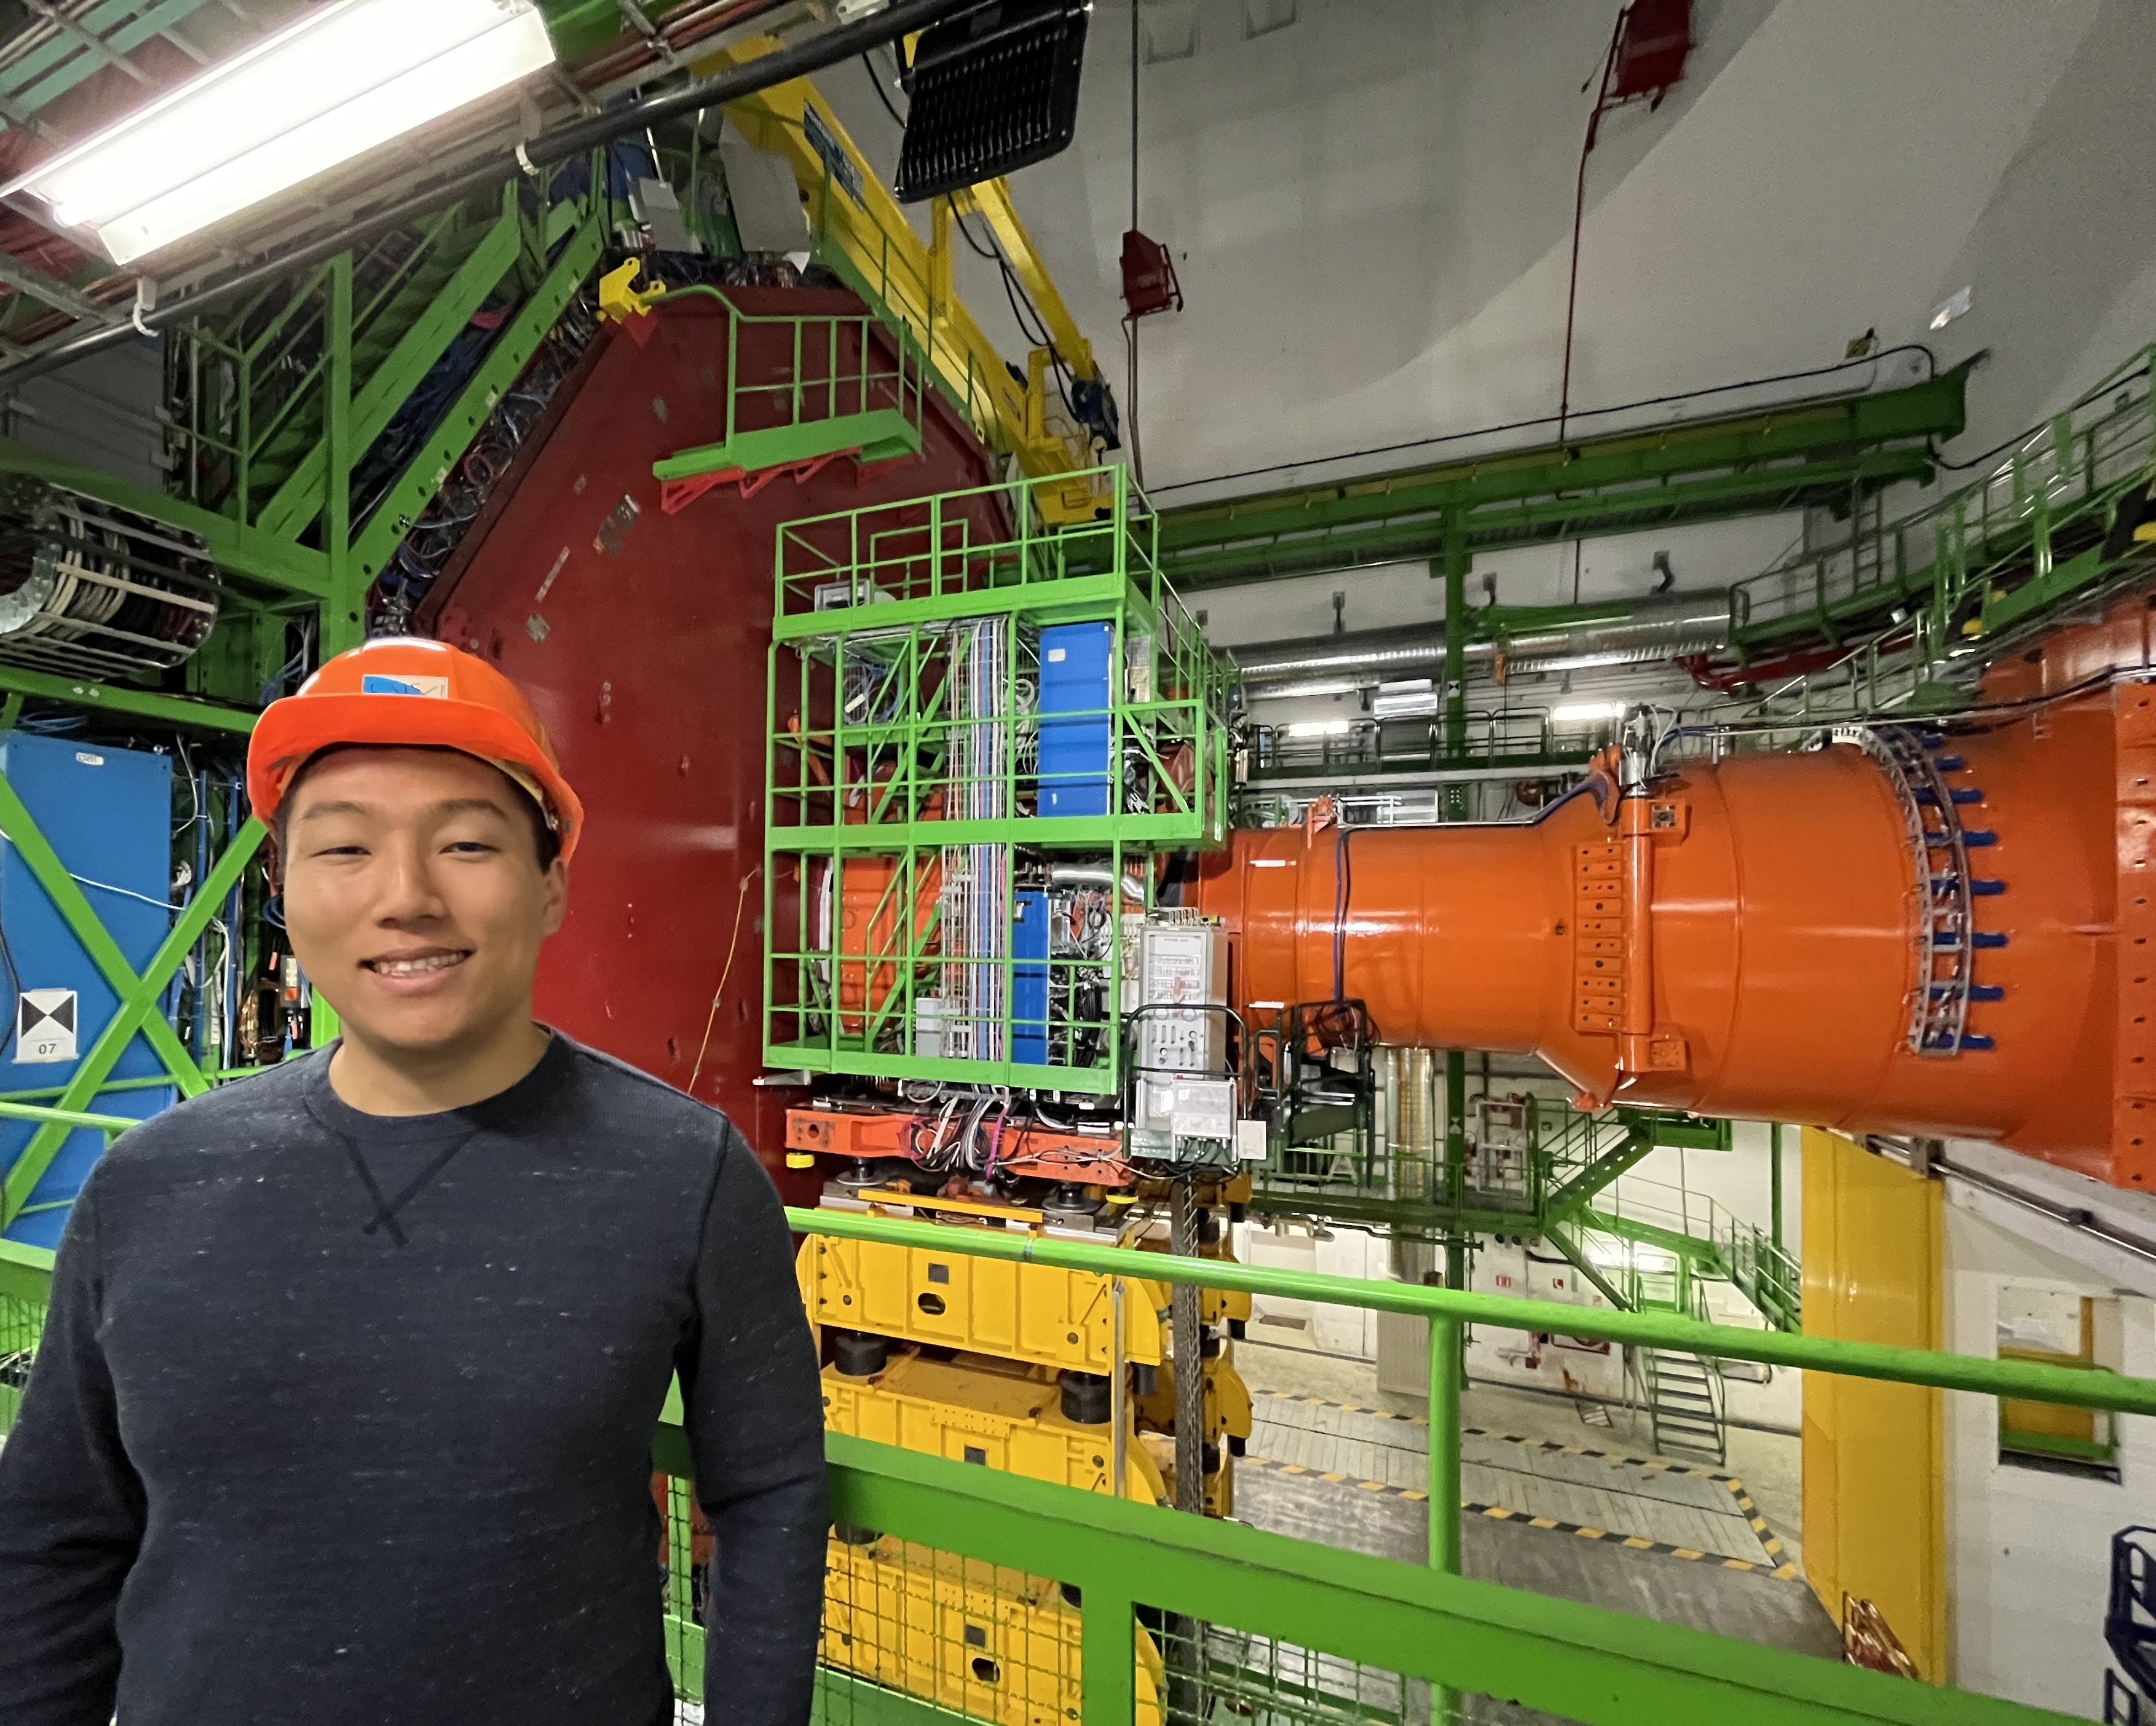
\includegraphics[width=0.4\textwidth,valign=c]{fig/cms/cms_jguiang.jpg}}
    \caption{
        The Compact Muon Solenoid in the closed configuration, pictured from the top (left) and side, with a physicist in the foreground for scale (right).
    }
    \label{fig:cms_jguiang}
\end{figure}

\clearpage

\section{The high lumonisity era}
\begin{figure}[!htb]
    \centering
    \subfloat[]{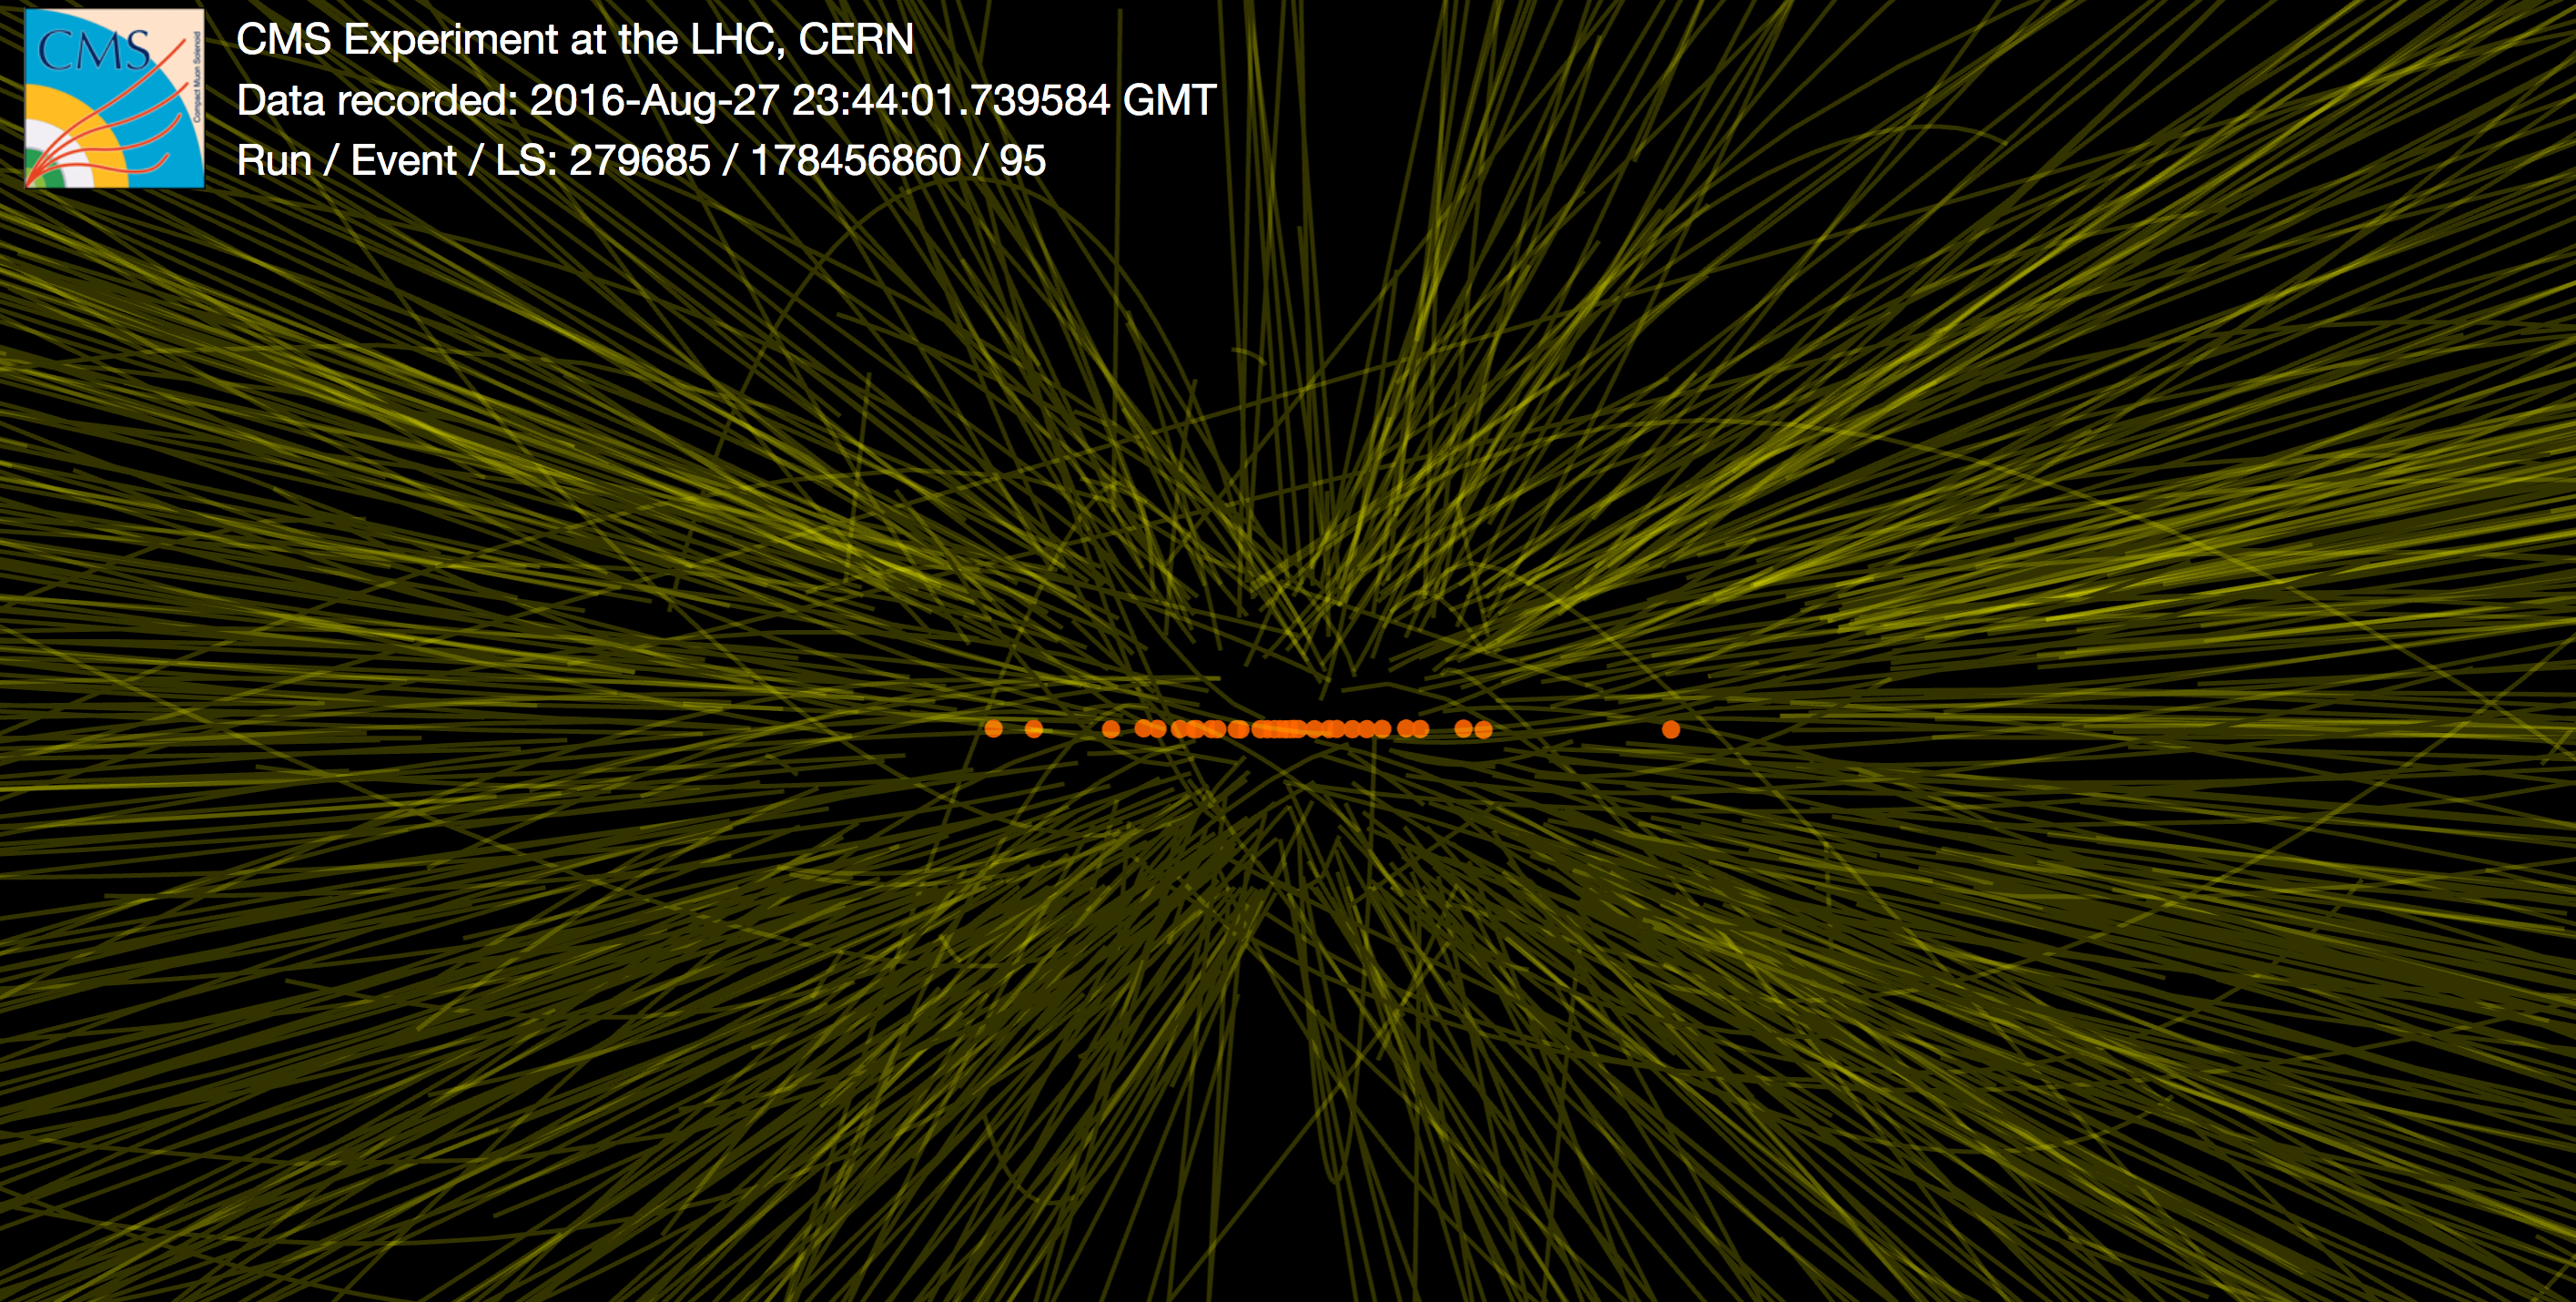
\includegraphics[width=0.45\linewidth]{fig/cms/high_PU_30vtx_side.png}\label{fig:normal_pu}}\qquad
    \subfloat[]{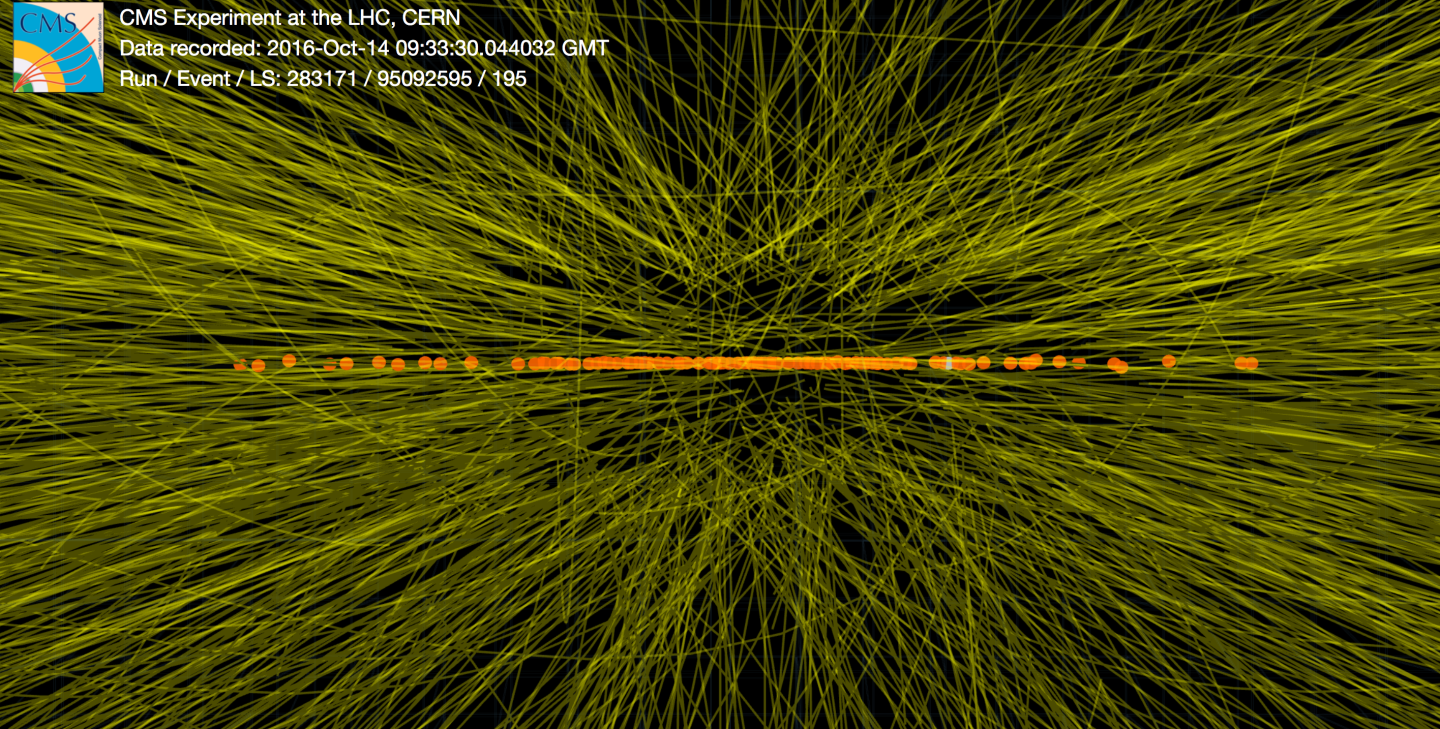
\includegraphics[width=0.45\linewidth]{fig/cms/high_PU_130vtx.png}\label{fig:high_pu}}
    \caption{
        A collision event with standard pileup (a) recorded at CMS in 2016 is shown next to an event with HL-LHC-like pileup (b) recorded at CMS in the same year, from Refs.~\cite{NormalPU2016, HighPU2016}.
        The dots are proton-proton collisions and the thin lines are the reconstructed particle tracks.
    }
    \label{fig:pileup}
\end{figure}
% What is HL?
%    - show pileup plots, maybe side AND 3D volume
% What upgrades?
%    - Give a basic overview: MTD, ph2 tracker, HGCAL
% What benefits does it bring?
%    - Find some papers...
